% slides/vapor.tex — vapor: tensores certificados, do termo ao registrador.
% 42 slides, Beamer 16:9. Compila com pdflatex (ou lualatex), só pacotes padrão
% do TeX Live: beamer, tikz, pgfplots, booktabs, amssymb.
%   pdflatex vapor.tex && pdflatex vapor.tex        (ou: make slides)
% Todo número neste arquivo foi medido no repositório (testes, exemplo SSM,
% bench/bench.exs, docs/bench/BENCH.md de 2026-10-01; a seção 7, das rodadas
% 0.8–0.14, de docs/bench/QUALITY.md, docs/FINANCAS.md e de
% `mix vapor.quality --only round14` de 2026-10-05) ou
% consultado na fonte citada no próprio slide.
\documentclass[aspectratio=169,10pt]{beamer}
\usepackage{iftex}
\ifPDFTeX\usepackage[utf8]{inputenc}\fi
% Latin Modern (T1) quando instalado; senão: pdfTeX usa Computer Modern com
% acentos compostos (vetorial), LuaTeX usa T1/EC (acentos nativos).
\IfFileExists{lmodern.sty}{\usepackage[T1]{fontenc}\usepackage{lmodern}}{\ifLuaTeX\usepackage[T1]{fontenc}\fi}
\usepackage{amsmath,amssymb}
\usepackage{booktabs,array}
\usepackage{tikz}
\usetikzlibrary{arrows.meta,positioning,calc,shapes.geometric,shapes.symbols,decorations.pathreplacing,fit,backgrounds,patterns}
\usepackage{pgfplots}
\pgfplotsset{compat=1.18}

% ---------------------------------------------------------------- paleta --
\definecolor{vnavy}{HTML}{0F172A}
\definecolor{vcyan}{HTML}{06B6D4}
\definecolor{vslate}{HTML}{334155}
\definecolor{vcoral}{HTML}{F43F5E}
\definecolor{vpaper}{HTML}{F8FAFC}
\definecolor{vmist}{HTML}{E2E8F0}
\definecolor{vink}{HTML}{1E293B}
\definecolor{vgreen}{HTML}{059669}
\definecolor{vamber}{HTML}{D97706}

% ------------------------------------------------------------------ tema --
\setbeamersize{text margin left=0.5cm,text margin right=0.5cm}
\setbeamercolor{background canvas}{bg=vpaper}
\setbeamercolor{normal text}{fg=vink}
\setbeamercolor{frametitle}{fg=white,bg=vnavy}
\setbeamercolor{structure}{fg=vcyan}
\setbeamercolor{alerted text}{fg=vcoral}
\setbeamerfont{frametitle}{size=\large,series=\bfseries}
\setbeamertemplate{navigation symbols}{}
\setbeamertemplate{itemize item}{\color{vcyan}$\blacktriangleright$}
\setbeamertemplate{frametitle}{%
  \nointerlineskip
  \begin{beamercolorbox}[wd=\paperwidth,ht=0.95cm,dp=0.35cm,leftskip=0.5cm,rightskip=0.5cm]{frametitle}%
    \usebeamerfont{frametitle}\insertframetitle\hfill
    {\normalfont\scriptsize\color{vcyan}\MakeUppercase{\insertsectionhead}}%
  \end{beamercolorbox}\vspace{0.1cm}}
\setbeamertemplate{footline}{%
  \hfill{\tiny\color{vslate}vapor\quad\insertframenumber\,/\,\inserttotalframenumber}\hspace*{0.6cm}\vspace*{0.18cm}}

% ------------------------------------------------------------- utilidades --
% A tese do slide: uma frase, sempre no mesmo lugar.
\newcommand{\tese}[1]{\par\vfill\noindent
  \begin{tikzpicture}
    \node[fill=vnavy,text=white,inner xsep=10pt,inner ysep=5pt,
          text width=\dimexpr\linewidth-21pt\relax,font=\small,align=left] (t) {#1};
    \fill[vcyan] (t.north west) rectangle ([xshift=4pt]t.south west);
  \end{tikzpicture}\par\vspace{0.05cm}}
\newcommand{\fonte}[1]{\par{\tiny\color{vslate!80}#1\par}}
\newcommand{\hl}[1]{{\color{vcyan!70!black}\textbf{#1}}}
\newcommand{\bad}[1]{{\color{vcoral}\textbf{#1}}}
\newcommand{\ok}{{\color{vgreen}$\checkmark$}}
\newcommand{\no}{{\color{vcoral}$\times$}}
\newcommand{\win}{\textcolor{vgreen}{\rule{5pt}{5pt}}\ }
\newcommand{\lose}{\textcolor{vcoral}{\rule{5pt}{5pt}}\ }

\tikzset{
  box/.style={draw=vslate!45,fill=white,rounded corners=3pt,line width=0.6pt,align=center,font=\scriptsize,inner sep=4pt},
  dark/.style={fill=vnavy,text=white,rounded corners=3pt,align=center,font=\scriptsize,inner sep=4pt},
  acc/.style={fill=vcyan!12,draw=vcyan,rounded corners=3pt,line width=0.7pt,align=center,font=\scriptsize,inner sep=4pt},
  badb/.style={fill=vcoral!10,draw=vcoral,rounded corners=3pt,line width=0.7pt,align=center,font=\scriptsize,inner sep=4pt},
  goodb/.style={fill=vgreen!10,draw=vgreen,rounded corners=3pt,line width=0.7pt,align=center,font=\scriptsize,inner sep=4pt},
  arr/.style={-{Stealth[length=5pt]},line width=0.8pt,draw=vslate},
  carr/.style={-{Stealth[length=5pt]},line width=1pt,draw=vcyan!80!black},
  rarr/.style={-{Stealth[length=5pt]},line width=1pt,draw=vcoral},
  lbl/.style={font=\tiny,text=vslate},
  boom/.style={starburst,starburst points=11,starburst point height=5pt,fill=vcoral,text=white,font=\tiny\bfseries,inner sep=1.5pt},
}

\title{vapor}
\date{5 de outubro de 2026}

\pgfplotsset{boxlegend/.style={legend image code/.code={\draw[#1,draw=none] (0cm,-0.08cm) rectangle (0.22cm,0.08cm);}}}
\begin{document}

% =========================================================================
% 1 — Título e roteiro
% =========================================================================
\begin{frame}[plain]
\begin{tikzpicture}[remember picture,overlay]
  \fill[vnavy] (current page.south west) rectangle (current page.north east);
  \coordinate (o) at ([xshift=1cm,yshift=-0.9cm]current page.north west);
  \node[anchor=north west,text=white,font=\fontsize{42}{46}\selectfont\bfseries,inner sep=0] at (o) {vapor};
  \node[anchor=north west,text=vcyan,font=\Large,inner sep=0] at ($(o)+(0.05,-1.55)$) {tensores certificados, do termo algébrico ao registrador};
  \node[anchor=north west,text=white!75,font=\small,text width=13.6cm,inner sep=0,align=left] at ($(o)+(0.05,-2.35)$)
    {Compilador e runtime de tensores em Elixir, \texttt{deps: []}. Emite \textbf{bits} para x86-64 (AVX2, AVX-512),
     AArch64, RVV 1.0 e SPIR-V, executa em processos isolados, sai de cada compilação com um certificado
     --- e sustenta um LLM inteiro com os mesmos bits em todo lugar.};
  % pipeline
  \foreach \t [count=\ix] in {termo simbólico,{reescrita exata}, {KIR + alocação}, {bits: 5 alvos}, {processo isolado}, {certificado Ed25519}} {
    \node[draw=vcyan,text=white,font=\scriptsize,rounded corners=2pt,minimum width=2.05cm,minimum height=0.62cm,align=center]
      (p\ix) at ($(o)+(1.0+2.33*\ix-2.33,-4.25)$) {\t};
  }
  \foreach \ix [evaluate=\ix as \j using int(\ix+1)] in {1,...,5} { \draw[-{Stealth[length=4pt]},vcyan,line width=0.8pt] (p\ix) -- (p\j); }
  % roteiro: as cinco perguntas
  \draw[white!35,line width=0.6pt] ($(o)+(0.7,-5.75)$) -- ($(o)+(12.9,-5.75)$);
  \foreach \n/\q/\s [count=\ix] in {1/Motivação/2--4, 2/Por quê/5--7, 3/Como/8--17, 4/{Ecossistema\\e HPC}/18--21, 5/{Agentes, RAG\\e ZK}/22--25, 6/Para quem/26--29, 7/{Rodadas\\0.8--0.13}/30--37, 8/Contribuição/38} {
    \node[circle,fill=vcyan,text=vnavy,font=\small\bfseries,minimum size=0.55cm,inner sep=0] (c\ix) at ($(o)+(0.7+1.74*\ix-1.74,-5.75)$) {\n};
    \node[text=white,font=\scriptsize\bfseries,anchor=north,align=center] at ($(c\ix.south)+(0,-0.05)$) {\q};
    \node[text=white!60,font=\tiny,anchor=north] at ($(c\ix.south)+(0,-0.72)$) {slides \s};
  }
  \node[anchor=south east,text=white!55,font=\tiny] at ([xshift=-0.6cm,yshift=0.35cm]current page.south east) {versão 0.13 · 5 de outubro de 2026};
\end{tikzpicture}
\end{frame}

% =========================================================================
\section{1 · Motivação}
% =========================================================================
\begin{frame}{Dor 1 --- gigabytes de pilha que ninguém audita}
\begin{columns}[T]
\begin{column}{0.62\textwidth}
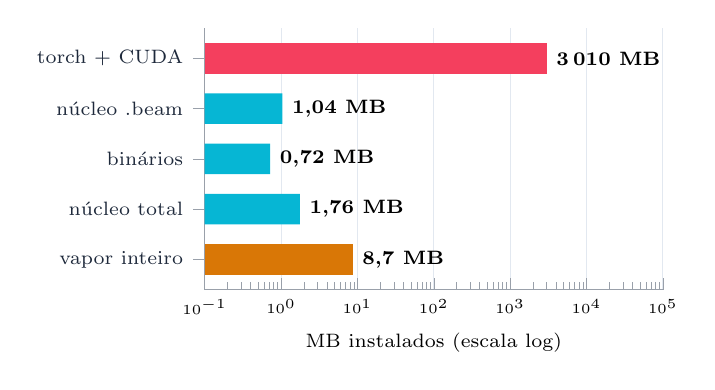
\begin{tikzpicture}
\begin{axis}[
  xbar, xmode=log, log origin x=infty, bar shift=0pt, bar width=11pt,
  width=7.4cm, height=4.9cm, xmin=0.1, xmax=100000,
  y dir=reverse, ytick={0,1,2,3,4}, ymin=-0.6, ymax=4.6,
  yticklabels={{torch + CUDA},{núcleo .beam},{binários},{núcleo total},{vapor inteiro}},
  yticklabel style={font=\scriptsize,text=vink,align=right},
  xlabel={MB instalados (escala log)}, xlabel style={font=\scriptsize},
  xticklabel style={font=\tiny}, axis line style={vslate!50}, tick style={vslate!50},
  axis x line*=bottom, axis y line*=left, xmajorgrids, grid style={vmist},
  point meta=explicit symbolic, nodes near coords, nodes near coords style={font=\scriptsize\bfseries,anchor=west},
  enlarge y limits=false]
  \addplot[fill=vcoral,draw=none] coordinates {(3010,0) [3\,010 MB]};
  \addplot[fill=vcyan,draw=none] coordinates {(1.04,1) [1,04 MB] (0.72,2) [0,72 MB] (1.76,3) [1,76 MB]};
  \addplot[fill=vamber,draw=none] coordinates {(8.66,4) [8,7 MB]};
\end{axis}
\end{tikzpicture}\\[-2pt]
\fonte{torch + CUDA: \texttt{torch==2.14.0} e 28 dependências (cp312, manylinux x86\_64), resolvidas com \texttt{pip install --dry-run} no PyPI em 28/09/2026, wheels comprimidos. vapor (0.13): \texttt{.beam} do núcleo (álgebra, compilação, emissores, verificação, runtime); binários = \texttt{vapor-worker} + \texttt{vapor-fabric}; inteiro = as 13 rodadas (modelos, documentos, mesas, finanças). Nenhum lado conta o runtime da linguagem (Python; Erlang/OTP = 32 MB aqui).}
\end{column}
\begin{column}{0.35\textwidth}
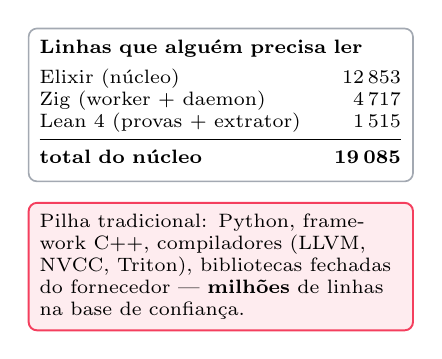
\begin{tikzpicture}
  \node[box,text width=4.6cm,align=left,font=\scriptsize] (a) {%
    \textbf{Linhas que alguém precisa ler}\\[3pt]
    \begin{tabular}{@{}lr@{}}
      Elixir (núcleo)             & 12\,853\\
      Zig (worker + daemon)      & 4\,717\\
      Lean 4 (provas + extrator) & 1\,515\\
      \midrule
      \textbf{total do núcleo}   & \textbf{19\,085}\\
    \end{tabular}};
  \node[badb,text width=4.6cm,align=left,below=0.25cm of a] {%
    Pilha tradicional: Python, framework C++, compiladores (LLVM, NVCC, Triton), bibliotecas
    fechadas do fornecedor --- \textbf{milhões} de linhas na base de confiança.};
\end{tikzpicture}
\end{column}
\end{columns}
\tese{Cada linha que executa é uma linha em que alguém confia. Escopo menor, sim --- mas \hl{$\sim$1\,700$\times$ menos bytes no núcleo} ($\sim$350$\times$ com as 13 rodadas) e uma base inteira que cabe numa revisão de código.}
\end{frame}

% -------------------------------------------------------------------------
\begin{frame}{Dor 2 --- o driver cai, o serviço inteiro cai junto}
\centering
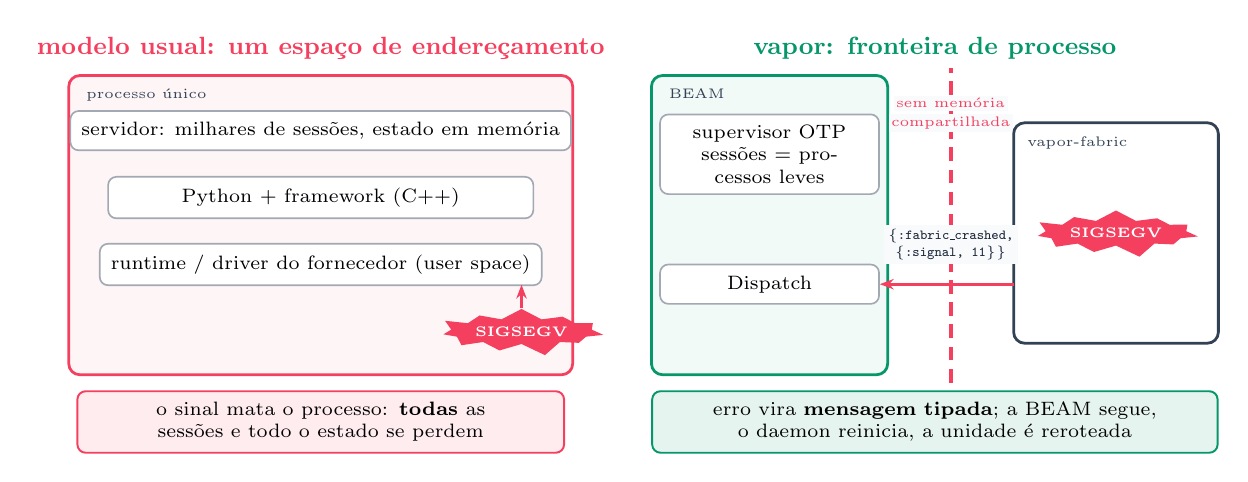
\begin{tikzpicture}
  % painel esquerdo: tudo no mesmo processo
  \node[font=\small\bfseries,text=vcoral] at (3.2,5.05) {modelo usual: um espaço de endereçamento};
  \draw[vcoral,line width=1pt,rounded corners=4pt,fill=vcoral!5] (0,0.9) rectangle (6.4,4.7);
  \node[lbl,anchor=north west] at (0.1,4.65) {processo único};
  \node[box,minimum width=5.4cm] (s1) at (3.2,4.0) {servidor: milhares de sessões, estado em memória};
  \node[box,minimum width=5.4cm] (s2) at (3.2,3.15) {Python + framework (C++)};
  \node[box,minimum width=5.4cm] (s3) at (3.2,2.3) {runtime / driver do fornecedor (user space)};
  \node[boom] (b1) at (5.75,1.45) {SIGSEGV};
  \draw[rarr] (b1.north) -- ++(0,0.3);
  \node[badb,text width=5.9cm] at (3.2,0.3) {o sinal mata o processo: \textbf{todas} as sessões e todo o estado se perdem};
  % painel direito: vapor
  \node[font=\small\bfseries,text=vgreen] at (11.0,5.05) {vapor: fronteira de processo};
  \draw[vgreen,line width=1pt,rounded corners=4pt,fill=vgreen!5] (7.4,0.9) rectangle (10.4,4.7);
  \node[lbl,anchor=north west] at (7.5,4.65) {BEAM};
  \node[box,text width=2.5cm] (sup) at (8.9,3.7) {supervisor OTP\\sessões = processos leves};
  \node[box,text width=2.5cm] (dis) at (8.9,2.05) {Dispatch};
  \draw[vcoral,line width=1.4pt,dash pattern=on 5pt off 3pt] (11.2,0.8) -- (11.2,4.8);
  \node[font=\tiny,text=vcoral,fill=vpaper,inner sep=1pt] at (11.2,4.35) {sem memória};
  \node[font=\tiny,text=vcoral,fill=vpaper,inner sep=1pt] at (11.2,4.1) {compartilhada};
  \draw[vslate,line width=1pt,rounded corners=4pt,fill=white] (12.0,1.3) rectangle (14.6,4.1);
  \node[lbl,anchor=north west] at (12.05,4.05) {vapor-fabric};
  \node[boom] (b2) at (13.3,2.7) {SIGSEGV};
  \draw[rarr] (12.0,2.05) -- (dis.east);
  \node[font=\tiny,text=vink,fill=vpaper,inner sep=1.5pt,align=center] at (11.2,2.55) {\texttt{\{:fabric\_crashed,}\\\texttt{\{:signal, 11\}\}}};
  \node[goodb,text width=6.9cm] at (11.0,0.3) {erro vira \textbf{mensagem tipada}; a BEAM segue, o daemon reinicia, a unidade é reroteada};
\end{tikzpicture}
\tese{Contenção não é \texttt{try/catch}: é um espaço de endereçamento separado. Fora dele, uma falha de driver é só um dado.}
\end{frame}

% -------------------------------------------------------------------------
\begin{frame}{Dor 3 --- a mesma soma, bits diferentes}
\centering
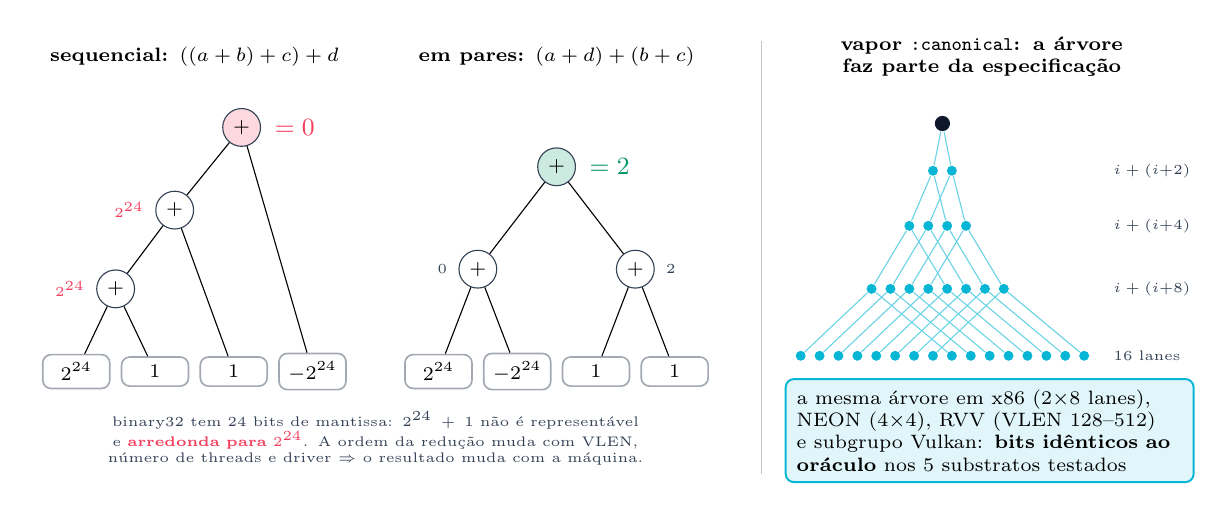
\begin{tikzpicture}[
  leaf/.style={box,minimum width=0.85cm,font=\scriptsize,inner sep=3pt},
  op/.style={circle,draw=vslate,fill=white,font=\scriptsize,inner sep=1pt,minimum size=0.48cm},
  val/.style={font=\tiny,text=vslate},
  dot/.style={circle,fill=vcyan,inner sep=0,minimum size=3.6pt}]
  % sequencial
  \node[font=\scriptsize\bfseries] at (2.0,4.0) {sequencial: $((a+b)+c)+d$};
  \node[leaf] (a) at (0.5,0) {$2^{24}$}; \node[leaf] (b) at (1.5,0) {$1$};
  \node[leaf] (c) at (2.5,0) {$1$};      \node[leaf] (d) at (3.5,0) {$-2^{24}$};
  \node[op] (ab) at (1.0,1.05) {$+$}; \node[val,anchor=east] at ($(ab.west)+(-0.02,0)$) {\bad{$2^{24}$}};
  \node[op] (abc) at (1.75,2.05) {$+$}; \node[val,anchor=east] at ($(abc.west)+(-0.02,0)$) {\bad{$2^{24}$}};
  \node[op,fill=vcoral!20] (r1) at (2.6,3.1) {$+$}; \node[font=\small\bfseries,text=vcoral,anchor=west] at ($(r1.east)+(0.05,0)$) {$=0$};
  \draw (a)--(ab) (b)--(ab) (ab)--(abc) (c)--(abc) (abc)--(r1) (d)--(r1);
  % pares
  \node[font=\scriptsize\bfseries] at (6.6,4.0) {em pares: $(a+d)+(b+c)$};
  \node[leaf] (a2) at (5.1,0) {$2^{24}$}; \node[leaf] (d2) at (6.1,0) {$-2^{24}$};
  \node[leaf] (b2) at (7.1,0) {$1$};      \node[leaf] (c2) at (8.1,0) {$1$};
  \node[op] (ad) at (5.6,1.3) {$+$}; \node[val,anchor=east] at ($(ad.west)+(-0.02,0)$) {$0$};
  \node[op] (bc) at (7.6,1.3) {$+$}; \node[val,anchor=west] at ($(bc.east)+(0.02,0)$) {$2$};
  \node[op,fill=vgreen!20] (r2) at (6.6,2.6) {$+$}; \node[font=\small\bfseries,text=vgreen,anchor=west] at ($(r2.east)+(0.05,0)$) {$=2$};
  \draw (a2)--(ad) (d2)--(ad) (b2)--(bc) (c2)--(bc) (ad)--(r2) (bc)--(r2);
  \node[lbl,text width=8.6cm,align=center] at (4.3,-0.85) {binary32 tem 24 bits de mantissa: $2^{24}+1$ não é representável e \bad{arredonda para $2^{24}$}.
    A ordem da redução muda com VLEN, número de threads e driver $\Rightarrow$ o resultado muda com a máquina.};
  % canônico
  \draw[vslate!30] (9.2,-1.3) -- (9.2,4.2);
  \node[font=\scriptsize\bfseries,text width=5.2cm,align=center] at (12.0,4.0) {vapor \texttt{:canonical}: a árvore faz parte da especificação};
  \begin{scope}[shift={(9.7,0.2)}]
  \foreach \ix in {0,...,15} { \node[dot] (l\ix) at (0.24*\ix,0) {}; }
  \foreach \ix in {0,...,7}  { \node[dot] (m\ix) at (0.24*\ix+0.9,0.85) {}; \draw[vcyan!60] (l\ix)--(m\ix); \pgfmathtruncatemacro{\k}{\ix+8}\draw[vcyan!60] (l\k)--(m\ix); }
  \foreach \ix in {0,...,3}  { \node[dot] (n\ix) at (0.24*\ix+1.38,1.65) {}; \draw[vcyan!60] (m\ix)--(n\ix); \pgfmathtruncatemacro{\k}{\ix+4}\draw[vcyan!60] (m\k)--(n\ix); }
  \foreach \ix in {0,1}      { \node[dot] (q\ix) at (0.24*\ix+1.68,2.35) {}; \draw[vcyan!60] (n\ix)--(q\ix); \pgfmathtruncatemacro{\k}{\ix+2}\draw[vcyan!60] (n\k)--(q\ix); }
  \node[dot,fill=vnavy,minimum size=5.5pt] (r) at (1.8,2.95) {}; \draw[vcyan!60] (q0)--(r) (q1)--(r);
  \node[lbl,anchor=west] at (3.85,0) {16 lanes};
  \node[lbl,anchor=west] at (3.85,0.85) {$i+(i{+}8)$};
  \node[lbl,anchor=west] at (3.85,1.65) {$i+(i{+}4)$};
  \node[lbl,anchor=west] at (3.85,2.35) {$i+(i{+}2)$};
  \end{scope}
  \node[acc,text width=4.9cm,align=left] at (12.1,-0.75) {a mesma árvore em x86 (2$\times$8 lanes), NEON (4$\times$4), RVV (VLEN 128--512) e subgrupo Vulkan: \textbf{bits idênticos ao oráculo} nos 5 substratos testados};
\end{tikzpicture}
\tese{Em ponto flutuante, $(a+b)+c \neq a+(b+c)$. Quem não fixa a ordem entrega um número que depende do hardware; o vapor fixa a ordem e \hl{testa a igualdade de bits} entre máquinas.}
\end{frame}

% =========================================================================
\section{2 · Por quê}
% =========================================================================
\begin{frame}{Cinco axiomas em vez de mais uma camada}
\centering
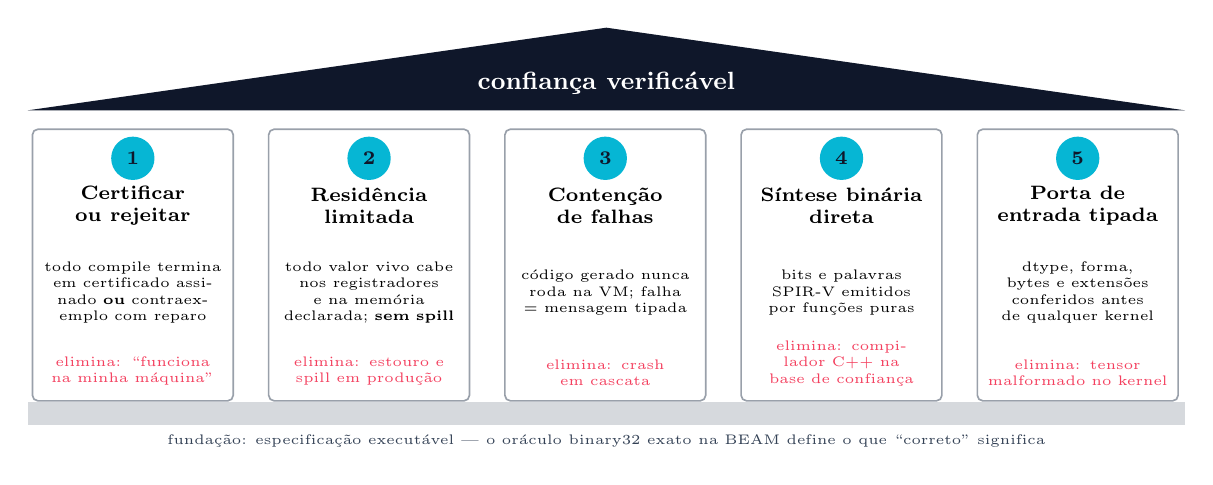
\begin{tikzpicture}[
  pil/.style={draw=vslate!50,fill=white,rounded corners=2pt,minimum width=2.55cm,minimum height=3.45cm,line width=0.6pt},
  num/.style={circle,fill=vcyan,text=vnavy,font=\scriptsize\bfseries,minimum size=0.55cm,inner sep=0}]
  \fill[vnavy] (0,4.0) -- (7.35,5.05) -- (14.7,4.0) -- cycle;
  \node[text=white,font=\small\bfseries] at (7.35,4.35) {confiança verificável};
  \foreach \n/\t/\d/\e [count=\ix] in {
      1/{Certificar\\ou rejeitar}/{todo compile termina em certificado assinado \textbf{ou} contraexemplo com reparo}/{``funciona na minha máquina''},
      2/{Residência\\limitada}/{todo valor vivo cabe nos registradores e na memória declarada; \textbf{sem spill}}/{estouro e spill em produção},
      3/{Contenção\\de falhas}/{código gerado nunca roda na VM; falha = mensagem tipada}/{crash em cascata},
      4/{Síntese binária\\direta}/{bits e palavras SPIR-V emitidos por funções puras}/{compilador C++ na base de confiança},
      5/{Porta de\\entrada tipada}/{dtype, forma, bytes e extensões conferidos antes de qualquer kernel}/{tensor malformado no kernel}} {
    \pgfmathsetmacro{\x}{3.0*\ix-3.0+0.05}
    \node[pil,anchor=south west] (P\ix) at (\x,0.3) {};
    \node[num] at ($(P\ix.north)+(0,-0.38)$) {\n};
    \node[font=\scriptsize\bfseries,align=center] at ($(P\ix.north)+(0,-0.98)$) {\t};
    \node[font=\tiny,text width=2.3cm,align=center] at ($(P\ix.center)+(0,-0.35)$) {\d};
    \node[font=\tiny,text=vcoral,text width=2.3cm,align=center,anchor=south] at ($(P\ix.south)+(0,0.08)$) {elimina: \e};
  }
  \fill[vslate!20] (0,0.0) rectangle (14.7,0.3);
  \node[font=\tiny,text=vslate] at (7.35,-0.2) {fundação: especificação executável --- o oráculo binary32 exato na BEAM define o que ``correto'' significa};
\end{tikzpicture}
\tese{Empacotar mais bibliotecas aumenta a superfície confiada sem verificação. Cada axioma \hl{remove uma classe inteira de falha} --- e é checado por máquina a cada compilação.}
\end{frame}

% -------------------------------------------------------------------------
\begin{frame}{Filosofia de segurança: provado, testado, confiado --- por escrito}
\begin{columns}[c]
\begin{column}{0.40\textwidth}
\centering
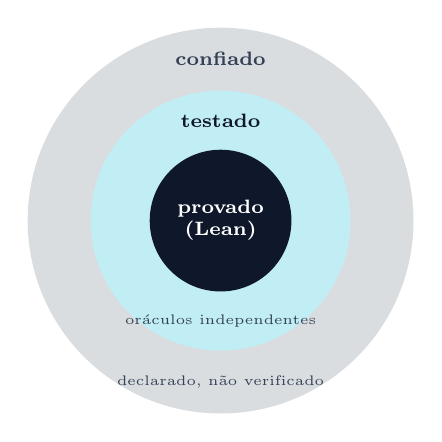
\begin{tikzpicture}
  \fill[vslate!18] (0,0) circle (2.45);
  \fill[vcyan!25]  (0,0) circle (1.65);
  \fill[vnavy]     (0,0) circle (0.9);
  \node[text=white,font=\scriptsize\bfseries,align=center] at (0,0) {provado\\(Lean)};
  \node[font=\scriptsize\bfseries,text=vnavy] at (0,1.27) {testado};
  \node[font=\scriptsize\bfseries,text=vslate] at (0,2.05) {confiado};
  \node[font=\tiny,text=vslate] at (0,-1.27) {oráculos independentes};
  \node[font=\tiny,text=vslate] at (0,-2.05) {declarado, não verificado};
\end{tikzpicture}
\end{column}
\begin{column}{0.58\textwidth}
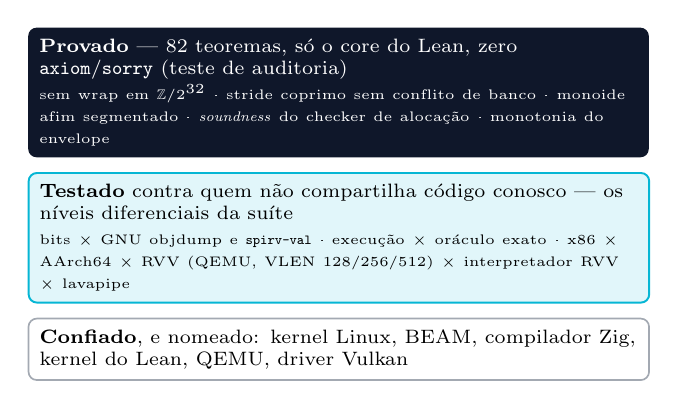
\begin{tikzpicture}
  \node[dark,text width=7.6cm,align=left,anchor=north west] (p) at (0,0) {%
    \textbf{Provado} --- 82 teoremas, só o core do Lean, zero \texttt{axiom}/\texttt{sorry} (teste de auditoria)\\[1pt]
    {\tiny sem wrap em $\mathbb{Z}/2^{32}$ \textperiodcentered{} stride coprimo sem conflito de banco \textperiodcentered{} monoide afim segmentado
     \textperiodcentered{} \emph{soundness} do checker de alocação \textperiodcentered{} monotonia do envelope}};
  \node[acc,text width=7.6cm,align=left,anchor=north west] (t) at ($(p.south west)+(0,-0.18)$) {%
    \textbf{Testado} contra quem não compartilha código conosco --- os níveis diferenciais da suíte\\[1pt]
    {\tiny bits $\times$ GNU objdump e \texttt{spirv-val} \textperiodcentered{} execução $\times$ oráculo exato \textperiodcentered{}
     x86 $\times$ AArch64 $\times$ RVV (QEMU, VLEN 128/256/512) $\times$ interpretador RVV $\times$ lavapipe}};
  \node[box,text width=7.6cm,align=left,anchor=north west] (c) at ($(t.south west)+(0,-0.18)$) {%
    \textbf{Confiado}, e nomeado: kernel Linux, BEAM, compilador Zig, kernel do Lean, QEMU, driver Vulkan};
\end{tikzpicture}
\end{column}
\end{columns}
\tese{Segurança começa por dizer o que \emph{não} está provado. O que não é provado é testado contra um oráculo independente; o que resta é \hl{declarado}, não escondido.}
\end{frame}

% -------------------------------------------------------------------------
\begin{frame}{Precisão: exata por construção, envelope quando rápida}
\centering
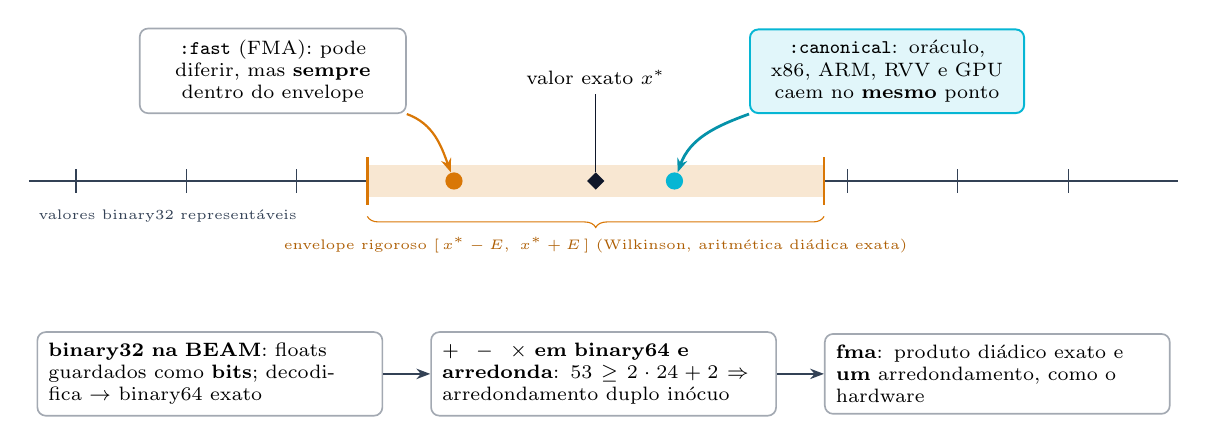
\begin{tikzpicture}
  % reta numérica
  \draw[vslate,line width=0.8pt] (0,2.2) -- (14.6,2.2);
  \foreach \x in {0.6,2.0,...,14.0} { \draw[vslate] (\x,2.05) -- (\x,2.35); }
  \node[lbl,anchor=west] at (0.0,1.75) {valores binary32 representáveis};
  % envelope
  \fill[vamber!18] (4.3,2.0) rectangle (10.1,2.4);
  \draw[vamber,line width=1pt] (4.3,1.9) -- (4.3,2.5) (10.1,1.9) -- (10.1,2.5);
  \draw[decorate,decoration={brace,amplitude=4pt,mirror},vamber] (4.3,1.75) -- (10.1,1.75)
    node[midway,below=4pt,font=\tiny,text=vamber!80!black] {envelope rigoroso $[\,x^\ast-E,\ x^\ast+E\,]$ (Wilkinson, aritmética diádica exata)};
  % exato
  \node[diamond,fill=vnavy,inner sep=1.6pt] (ex) at (7.2,2.2) {};
  \node[font=\scriptsize,anchor=south] at (7.2,3.3) {valor exato $x^\ast$};
  \draw[vnavy] (7.2,3.3) -- (ex);
  % canônico
  \node[circle,fill=vcyan,inner sep=2.2pt] (cn) at (8.2,2.2) {};
  \node[acc,anchor=south,text width=3.2cm] (cl) at (10.9,3.05) {\texttt{:canonical}: oráculo, x86, ARM, RVV e GPU caem no \textbf{mesmo} ponto};
  \draw[carr] (cl.south west) to[out=200,in=70] (cn);
  % rápido
  \node[circle,fill=vamber,inner sep=2.2pt] (fs) at (5.4,2.2) {};
  \node[box,anchor=south,text width=3.1cm] (fl) at (3.1,3.05) {\texttt{:fast} (FMA): pode diferir, mas \textbf{sempre} dentro do envelope};
  \draw[arr,draw=vamber] (fl.south east) to[out=-20,in=110] (fs);
  % como o oráculo é exato
  \node[box,text width=4.1cm,align=left] (o1) at (2.3,-0.25) {\textbf{binary32 na BEAM}: floats guardados como \textbf{bits}; decodifica $\to$ binary64 exato};
  \node[box,text width=4.1cm,align=left] (o2) at (7.3,-0.25) {\textbf{$+\ -\ \times$ em binary64 e arredonda}: $53 \ge 2\cdot 24+2 \Rightarrow$ arredondamento duplo inócuo};
  \node[box,text width=4.1cm,align=left] (o3) at (12.3,-0.25) {\textbf{fma}: produto diádico exato e \textbf{um} arredondamento, como o hardware};
  \draw[arr] (o1) -- (o2); \draw[arr] (o2) -- (o3);
\end{tikzpicture}
\tese{Dois contratos explícitos: \texttt{:canonical} = \hl{os mesmos bits do oráculo exato em toda máquina}; \texttt{:fast} = qualquer resultado \hl{dentro de um envelope provado}, decidido por código extraído do Lean.}
\end{frame}

% =========================================================================
\section{3 · Como}
% =========================================================================
\begin{frame}{Arquitetura tripartite: decidir, executar, sobreviver}
\centering
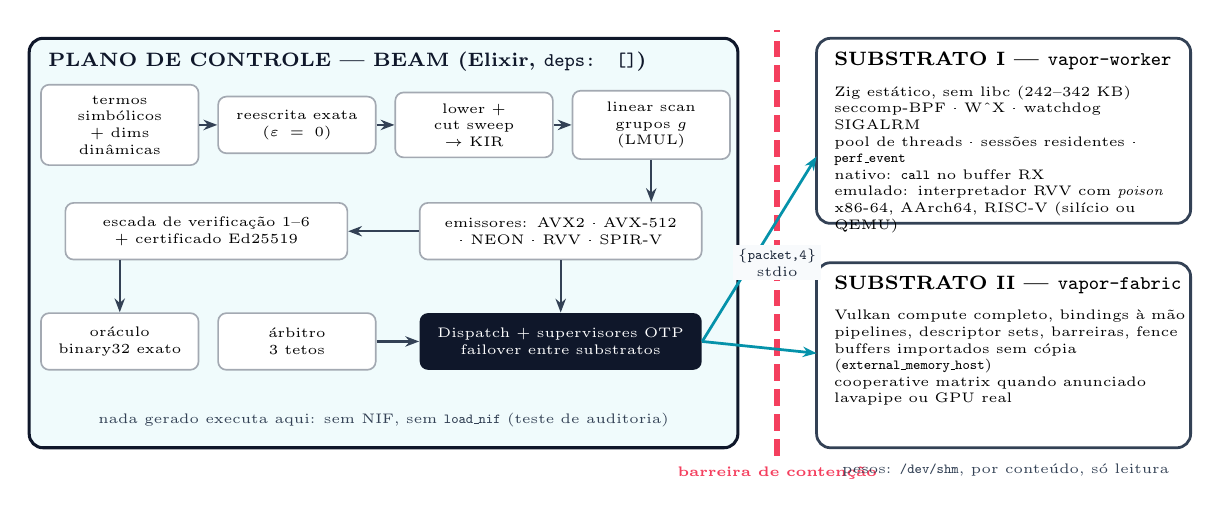
\begin{tikzpicture}[n/.style={box,font=\tiny,text width=1.72cm,minimum height=0.72cm}]
  % plano de controle
  \draw[vnavy,line width=1.1pt,rounded corners=5pt,fill=vcyan!6] (0,0) rectangle (9.0,5.2);
  \node[anchor=north west,font=\scriptsize\bfseries,text=vnavy] at (0.12,5.15) {PLANO DE CONTROLE --- BEAM (Elixir, \texttt{deps: []})};
  \node[n] (t1) at (1.15,4.1) {termos simbólicos\\+ dims dinâmicas};
  \node[n] (t2) at (3.4,4.1) {reescrita exata\\($\varepsilon = 0$)};
  \node[n] (t3) at (5.65,4.1) {lower + cut sweep\\$\to$ KIR};
  \node[n] (t4) at (7.9,4.1) {linear scan\\grupos $g$ (LMUL)};
  \node[n,text width=3.3cm] (t5) at (6.75,2.75) {emissores: AVX2 \textperiodcentered{} AVX-512 \textperiodcentered{} NEON \textperiodcentered{} RVV \textperiodcentered{} SPIR-V};
  \node[n,text width=3.3cm] (t6) at (2.25,2.75) {escada de verificação 1--6\\+ certificado Ed25519};
  \node[n] (t7) at (1.15,1.35) {oráculo\\binary32 exato};
  \node[n] (t8) at (3.4,1.35) {árbitro\\3 tetos};
  \node[dark,font=\tiny,text width=3.3cm,minimum height=0.72cm] (t9) at (6.75,1.35) {Dispatch + supervisores OTP\\failover entre substratos};
  \draw[arr] (t1)--(t2); \draw[arr] (t2)--(t3); \draw[arr] (t3)--(t4); \draw[arr] (t4)--(t4 |- t5.north);
  \draw[arr] (t5)--(t6); \draw[arr] (t6.south -| t7)--(t7); \draw[arr] (t8)--(t9); \draw[arr] (t5)--(t9);
  \node[lbl] at (4.5,0.35) {nada gerado executa aqui: sem NIF, sem \texttt{load\_nif} (teste de auditoria)};
  % barreira
  \draw[vcoral,line width=2pt,dash pattern=on 6pt off 3pt] (9.5,-0.1) -- (9.5,5.3);
  \node[font=\tiny\bfseries,text=vcoral,anchor=north] at (9.5,-0.12) {barreira de contenção};
  % substrato I
  \draw[vslate,line width=1pt,rounded corners=5pt,fill=white] (10.0,2.85) rectangle (14.75,5.2);
  \node[anchor=north west,font=\scriptsize\bfseries] at (10.1,5.15) {SUBSTRATO I --- \texttt{vapor-worker}};
  \node[font=\tiny,text width=4.5cm,align=left,anchor=north west] at (10.1,4.72) {Zig estático, sem libc (242--342 KB)\\
    seccomp-BPF \textperiodcentered{} W\^{}X \textperiodcentered{} watchdog SIGALRM\\
    pool de threads \textperiodcentered{} sessões residentes \textperiodcentered{} \texttt{perf\_event}\\
    nativo: \texttt{call} no buffer RX\\
    emulado: interpretador RVV com \emph{poison}\\
    x86-64, AArch64, RISC-V (silício ou QEMU)};
  % substrato II
  \draw[vslate,line width=1pt,rounded corners=5pt,fill=white] (10.0,0.0) rectangle (14.75,2.35);
  \node[anchor=north west,font=\scriptsize\bfseries] at (10.1,2.3) {SUBSTRATO II --- \texttt{vapor-fabric}};
  \node[font=\tiny,text width=4.5cm,align=left,anchor=north west] at (10.1,1.87) {Vulkan compute completo, bindings à mão\\
    pipelines, descriptor sets, barreiras, fence\\
    buffers importados sem cópia (\texttt{external\_memory\_host})\\
    cooperative matrix quando anunciado\\
    lavapipe ou GPU real};
  \draw[carr] (t9.east) -- (10.0,3.7);
  \draw[carr] (t9.east) -- (10.0,1.2);
  \node[font=\tiny,text=vink,fill=vpaper,inner sep=1.5pt,align=center] at (9.5,2.35) {\texttt{\{packet,4\}}\\stdio};
  \node[font=\tiny,text=vslate,anchor=north] at (12.4,-0.08) {pesos: \texttt{/dev/shm}, por conteúdo, só leitura};
\end{tikzpicture}
\tese{A BEAM \hl{decide, verifica e supervisiona}; os substratos \hl{só executam} --- e podem morrer. Nenhum byte gerado roda no espaço de endereçamento da VM.}
\end{frame}

% -------------------------------------------------------------------------
\begin{frame}{Ponta a ponta: do arquivo de pesos ao registrador e ao token}
\centering
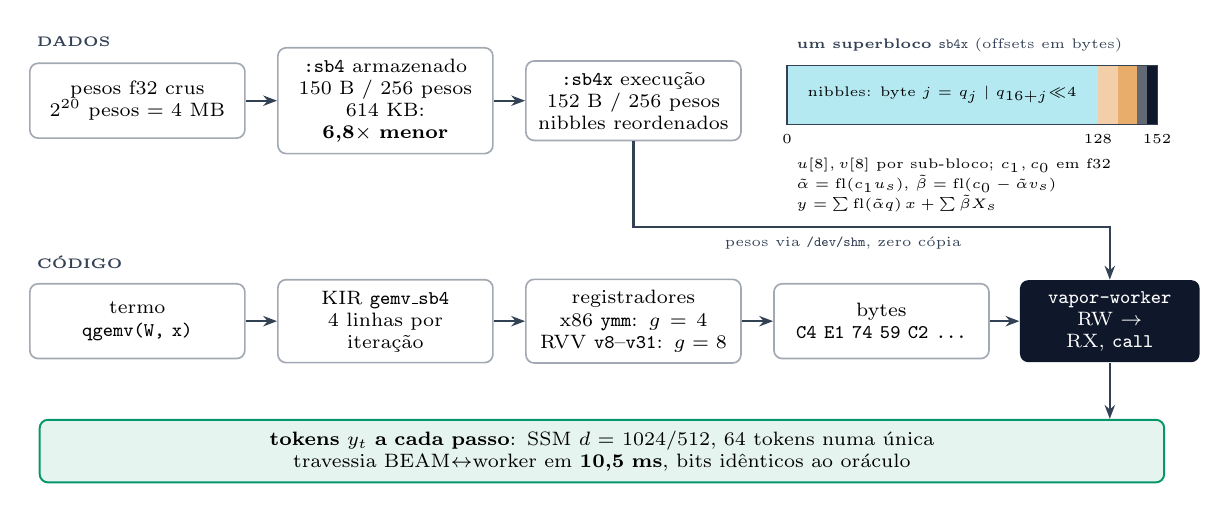
\begin{tikzpicture}[n/.style={box,minimum height=0.95cm,text width=2.45cm}]
  % trilha de dados
  \node[lbl,anchor=west] at (-0.1,5.1) {\textbf{DADOS}};
  \node[n] (d1) at (1.3,4.35) {pesos f32 crus\\$2^{20}$ pesos = 4 MB};
  \node[n] (d2) at (4.45,4.35) {\texttt{:sb4} armazenado\\150 B / 256 pesos\\614 KB: \textbf{6,8$\times$ menor}};
  \node[n] (d3) at (7.6,4.35) {\texttt{:sb4x} execução\\152 B / 256 pesos\\nibbles reordenados};
  \draw[arr] (d1)--(d2); \draw[arr] (d2)--(d3);
  % layout sb4x
  \begin{scope}[shift={(9.55,4.05)}]
    \node[lbl,anchor=south west] at (0,0.8) {\textbf{um superbloco \texttt{sb4x}} (offsets em bytes)};
    \fill[vcyan!30] (0,0) rectangle (3.95,0.75);
    \node[font=\tiny,align=center] at (1.97,0.375) {nibbles: byte $j$ = $q_j \mid q_{16+j}{\ll}4$};
    \fill[vamber!35] (3.95,0) rectangle (4.2,0.75);
    \fill[vamber!60] (4.2,0) rectangle (4.45,0.75);
    \fill[vnavy!65] (4.45,0) rectangle (4.575,0.75);
    \fill[vnavy] (4.575,0) rectangle (4.7,0.75);
    \draw[vslate] (0,0) rectangle (4.7,0.75);
    \foreach \x/\l in {0/0,3.95/128,4.7/152} { \node[font=\tiny,anchor=north] at (\x,0) {\l}; }
    \node[font=\tiny,anchor=north west,text width=4.9cm,align=left] at (0,-0.3) {$u[8], v[8]$ por sub-bloco; $c_1, c_0$ em f32\\
      $\tilde\alpha=\mathrm{fl}(c_1u_s)$,\ $\tilde\beta=\mathrm{fl}(c_0-\tilde\alpha v_s)$\\ $y=\sum \mathrm{fl}(\tilde\alpha q)\,x + \sum \tilde\beta X_s$};
  \end{scope}
  % trilha de código
  \node[lbl,anchor=west] at (-0.1,2.3) {\textbf{CÓDIGO}};
  \node[n] (c1) at (1.3,1.55) {termo\\\texttt{qgemv(W, x)}};
  \node[n] (c2) at (4.45,1.55) {KIR \texttt{gemv\_sb4}\\4 linhas por iteração};
  \node[n] (c3) at (7.6,1.55) {registradores\\x86 \texttt{ymm}: $g=4$\\RVV \texttt{v8}--\texttt{v31}: $g=8$};
  \node[n] (c4) at (10.75,1.55) {bytes\\\texttt{C4 E1 74 59 C2 \ldots}};
  \draw[arr] (c1)--(c2); \draw[arr] (c2)--(c3); \draw[arr] (c3)--(c4);
  \node[dark,text width=2.0cm,minimum height=0.95cm] (w) at (13.65,1.55) {\texttt{vapor-worker}\\RW $\to$ RX, \texttt{call}};
  \draw[arr] (c4)--(w);
  \draw[arr] (d3.south) |- (13.65,2.75) node[pos=0.72,below,lbl] {pesos via \texttt{/dev/shm}, zero cópia} -- (w.north);
  \node[goodb,text width=14.0cm] (tok) at (7.2,-0.1) {\textbf{tokens $y_t$ a cada passo}: SSM $d$ = 1024/512, 64 tokens numa única travessia BEAM$\leftrightarrow$worker em \textbf{10,5 ms}, bits idênticos ao oráculo};
  \draw[arr] (w.south) -- (w.south |- tok.north);
\end{tikzpicture}
\tese{Um caminho só, visível de ponta a ponta: \hl{sem C, sem LLVM, sem runtime do fornecedor na CPU}. Os pesos cruzam uma vez, por mapeamento; os tokens voltam em fluxo.}
\end{frame}

% -------------------------------------------------------------------------
\begin{frame}{Bits sem toolchain: a mesma multiplicação vetorial em três ISAs}
\centering
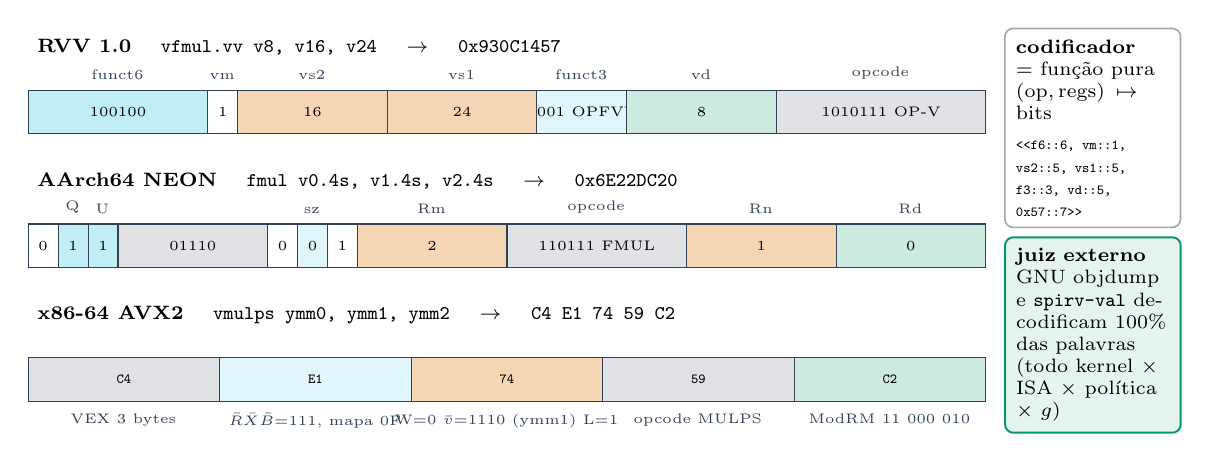
\begin{tikzpicture}[fld/.style={draw=vslate,font=\tiny,align=center,inner sep=0,minimum height=0.55cm}]
  \def\u{0.38}
  % --- RVV
  \node[anchor=west,font=\scriptsize] at (0,4.65) {\textbf{RVV 1.0} \quad \texttt{vfmul.vv v8, v16, v24} \quad $\to$ \quad \texttt{0x930C1457}};
  \foreach \xo/\w/\l/\v/\c in {0/6/funct6/100100/vcyan!25, 6/1/vm/1/white, 7/5/vs2/16/vamber!30, 12/5/vs1/24/vamber!30, 17/3/funct3/{001 OPFVV}/vcyan!12, 20/5/vd/8/vgreen!20, 25/7/opcode/{1010111 OP-V}/vslate!15} {
    \node[fld,fill=\c,minimum width={\w*\u cm},anchor=south west] at (\xo*\u,3.55) {\v};
    \node[font=\tiny,text=vslate,anchor=south] at ({(\xo+\w/2)*\u},4.12) {\l};
  }
  % --- AArch64
  \node[anchor=west,font=\scriptsize] at (0,2.95) {\textbf{AArch64 NEON} \quad \texttt{fmul v0.4s, v1.4s, v2.4s} \quad $\to$ \quad \texttt{0x6E22DC20}};
  \foreach \xo/\w/\l/\v/\c in {0/1//0/white, 1/1/Q/1/vcyan!25, 2/1/U/1/vcyan!25, 3/5//01110/vslate!15, 8/1//0/white, 9/1/sz/0/vcyan!12, 10/1//1/white, 11/5/Rm/2/vamber!30, 16/6/opcode/{110111 FMUL}/vslate!15, 22/5/Rn/1/vamber!30, 27/5/Rd/0/vgreen!20} {
    \node[fld,fill=\c,minimum width={\w*\u cm},anchor=south west] at (\xo*\u,1.85) {\v};
    \node[font=\tiny,text=vslate,anchor=south] at ({(\xo+\w/2)*\u},2.42) {\l};
  }
  % --- x86-64
  \node[anchor=west,font=\scriptsize] at (0,1.25) {\textbf{x86-64 AVX2} \quad \texttt{vmulps ymm0, ymm1, ymm2} \quad $\to$ \quad \texttt{C4 E1 74 59 C2}};
  \foreach \v/\l/\c [count=\ix] in {C4/{VEX 3 bytes}/vslate!15, E1/{$\bar R\bar X\bar B$=111, mapa 0F}/vcyan!12, 74/{W=0 $\bar v$=1110 (ymm1) L=1}/vamber!30, 59/{opcode MULPS}/vslate!15, C2/{ModRM 11 000 010}/vgreen!20} {
    \node[fld,fill=\c,minimum width=2.432cm,anchor=south west] at ({(\ix-1)*2.432},0.15) {\texttt{\v}};
    \node[font=\tiny,text=vslate,anchor=north] at ({(\ix-1)*2.432+1.216},0.12) {\l};
  }
  % lado direito
  \node[box,text width=1.95cm,align=left,anchor=north west] at (12.4,4.9) {\textbf{codificador}\\= função pura\\$(\text{op}, \text{regs}) \mapsto$ bits\\[3pt]
    {\tiny \texttt{<<f6::6, vm::1, vs2::5, vs1::5, f3::3, vd::5, 0x57::7>>}}};
  \node[goodb,text width=1.95cm,align=left,anchor=north west] at (12.4,2.25) {\textbf{juiz externo}\\GNU objdump e \texttt{spirv-val} decodificam 100\% das palavras (todo kernel $\times$ ISA $\times$ política $\times$ $g$)};
\end{tikzpicture}
\tese{Sem assembler externo, a \hl{especificação da ISA é o único contrato} --- e uma ferramenta que não compartilha código conosco é o árbitro. SPIR-V segue igual: palavras de 32 bits, \texttt{NoContraction} para fixar a ordem.}
\end{frame}

% -------------------------------------------------------------------------
\begin{frame}{Alocação: linear scan com grupos (LMUL), sem spill, verificada}
\centering
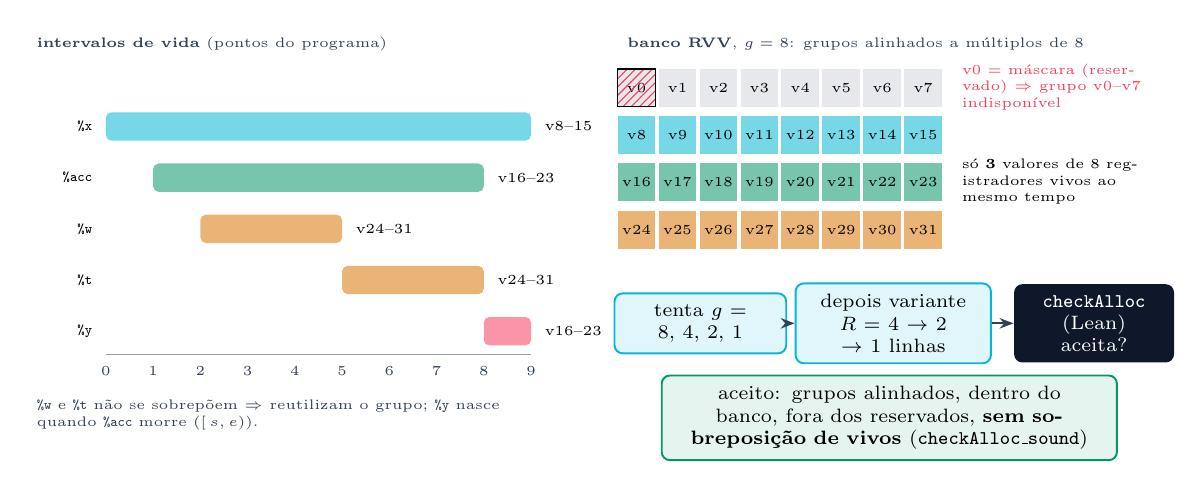
\begin{tikzpicture}
  % intervalos de vida
  \node[lbl,anchor=west] at (0,4.85) {\textbf{intervalos de vida} (pontos do programa)};
  \draw[vslate!50] (1.0,0.9) -- (6.4,0.9);
  \foreach \t in {0,...,9} { \node[font=\tiny,text=vslate] at (1.0+0.6*\t,0.7) {\t}; }
  \foreach \n/\s/\e/\c/\r [count=\ix] in {x/0/9/vcyan/{v8--15},acc/1/8/vgreen/{v16--23},w/2/5/vamber/{v24--31},t/5/8/vamber/{v24--31},y/8/9/vcoral/{v16--23}} {
    \pgfmathsetmacro{\y}{4.45-0.65*\ix}
    \fill[\c!55,rounded corners=2pt] ({1.0+0.6*\s},\y-0.18) rectangle ({1.0+0.6*\e},\y+0.18);
    \node[font=\tiny,anchor=east] at (0.95,\y) {\texttt{\%\n}};
    \node[font=\tiny,anchor=west] at ({1.05+0.6*\e},\y) {\r};
  }
  \node[lbl,text width=6.2cm,align=left,anchor=north west] at (0.0,0.45) {\texttt{\%w} e \texttt{\%t} não se sobrepõem $\Rightarrow$ reutilizam o grupo; \texttt{\%y} nasce quando \texttt{\%acc} morre ($[\,s, e)$).};
  % banco de registradores RVV
  \node[lbl,anchor=west] at (7.5,4.85) {\textbf{banco RVV}, $g=8$: grupos alinhados a múltiplos de 8};
  \foreach \r in {0,...,31} {
    \pgfmathtruncatemacro{\row}{\r/8} \pgfmathtruncatemacro{\col}{mod(\r,8)}
    \ifcase\row \def\cc{vslate!12}\or \def\cc{vcyan!55}\or \def\cc{vgreen!55}\or \def\cc{vamber!55}\fi
    \fill[\cc] ({7.5+0.52*\col},{4.05-0.6*\row}) rectangle ++(0.48,0.48);
    \node[font=\tiny] at ({7.74+0.52*\col},{4.29-0.6*\row}) {v\r};
  }
  \draw[pattern=north east lines,pattern color=vcoral] (7.5,4.05) rectangle ++(0.48,0.48);
  \node[font=\tiny,text=vcoral,anchor=west,text width=2.4cm,align=left] at (11.75,4.3) {v0 = máscara (reservado) $\Rightarrow$ grupo v0--v7 indisponível};
  \node[font=\tiny,anchor=west,text width=2.4cm,align=left] at (11.75,3.1) {só \textbf{3} valores de 8 registradores vivos ao mesmo tempo};
  % cadeia de fallback
  \node[acc,text width=1.9cm] (f1) at (8.55,1.3) {tenta $g$ = 8, 4, 2, 1};
  \node[acc,text width=2.2cm] (f2) at (11.0,1.3) {depois variante\\$R$ = 4 $\to$ 2 $\to$ 1 linhas};
  \node[dark,text width=1.75cm] (f3) at (13.55,1.3) {\texttt{checkAlloc}\\(Lean) aceita?};
  \draw[arr] (f1)--(f2); \draw[arr] (f2)--(f3);
  \node[goodb,text width=5.5cm] at (10.95,0.1) {aceito: grupos alinhados, dentro do banco, fora dos reservados, \textbf{sem sobreposição de vivos} (\texttt{checkAlloc\_sound})};
\end{tikzpicture}
\tese{Selecionar antes de alocar, nunca emitir spill, e aceitar só o que um \hl{checker provado} aceita: o alocador é heurístico e pode errar --- o código emitido não herda o erro.}
\end{frame}

% -------------------------------------------------------------------------
\begin{frame}{Isolamento em camadas: o pior código vira um erro tipado}
\begin{columns}[c]
\begin{column}{0.45\textwidth}
\centering
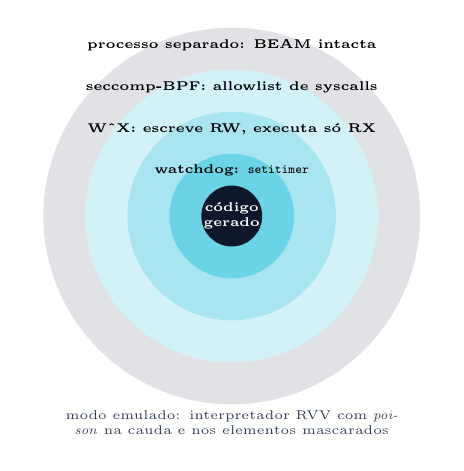
\begin{tikzpicture}[scale=0.92,transform shape]
  \foreach \r/\c/\t/\y in {2.6/vslate!15/{processo separado: BEAM intacta}/2.35,
                           2.02/vcyan!18/{seccomp-BPF: allowlist de syscalls}/1.77,
                           1.44/vcyan!35/{W\^{}X: escreve RW, executa só RX}/1.19,
                           0.86/vcyan!60/{watchdog: \texttt{setitimer}}/0.63} {
    \fill[\c] (0,0) circle (\r);
    \node[font=\tiny\bfseries] at (0,\y) {\t};
  }
  \fill[vnavy] (0,0) circle (0.42);
  \node[text=white,font=\tiny\bfseries,align=center] at (0,0) {código\\gerado};
  \node[font=\tiny,text=vslate,text width=5.4cm,align=center] at (0,-2.85) {modo emulado: interpretador RVV com \emph{poison} na cauda e nos elementos mascarados};
\end{tikzpicture}
\end{column}
\begin{column}{0.52\textwidth}
\scriptsize
\renewcommand{\arraystretch}{1.35}
\begin{tabular}{@{}>{\raggedright\arraybackslash}p{2.0cm}p{1.2cm}>{\raggedright\arraybackslash}p{3.75cm}@{}}
\toprule
\textbf{falha injetada} & \textbf{sinal} & \textbf{o que a BEAM recebe}\\
\midrule
instrução ilegal & SIGILL & \texttt{\{:worker\_crashed, \{:signal, :sigill\}\}}\\
acesso inválido & SIGSEGV & \texttt{\{:worker\_crashed, \{:signal, :sigsegv\}\}}\\
laço infinito (\texttt{EB FE}) & SIGALRM & \texttt{\{:worker\_crashed, \{:signal, :sigalrm\}\}}\\
syscall proibida & SIGSYS & \texttt{\{:worker\_crashed, \{:signal, :sigsys\}\}}\\
driver Vulkan & SIGSEGV & \texttt{\{:fabric\_crashed, \{:signal, 11\}\}}\\
\bottomrule
\end{tabular}\\[6pt]
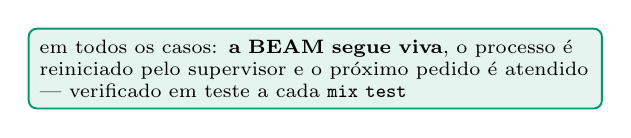
\begin{tikzpicture}
  \node[goodb,text width=7.0cm,align=left] {em todos os casos: \textbf{a BEAM segue viva}, o processo é reiniciado pelo supervisor e o próximo pedido é atendido --- verificado em teste a cada \texttt{mix test}};
\end{tikzpicture}
\end{column}
\end{columns}
\tese{Defesa em profundidade com uma regra simples: \hl{qualquer} coisa que o código gerado faça de errado termina num sinal, e todo sinal termina numa \hl{mensagem}.}
\end{frame}

% -------------------------------------------------------------------------
\begin{frame}{Auto-recuperação: a GPU falha no meio do serviço}
\centering
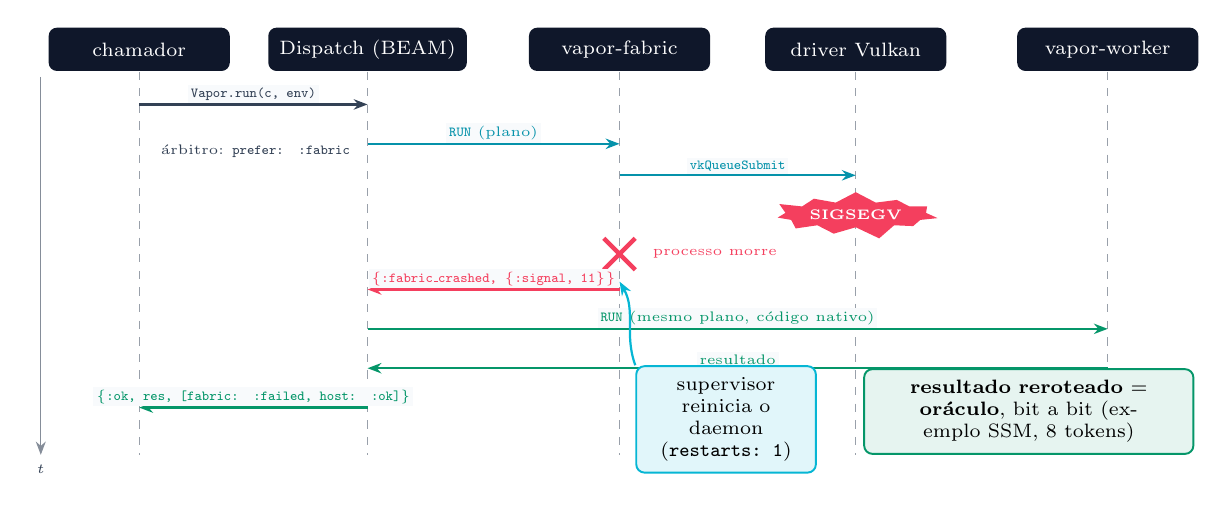
\begin{tikzpicture}[ll/.style={dark,minimum width=2.3cm,minimum height=0.55cm},
                    msg/.style={-{Stealth[length=5pt]},line width=0.8pt},
                    mt/.style={font=\tiny,fill=vpaper,inner sep=1pt}]
  \foreach \x/\n/\t in {0.9/C/chamador,3.8/D/{Dispatch (BEAM)},7.0/F/vapor-fabric,10.0/V/{driver Vulkan},13.2/W/vapor-worker} {
    \node[ll] (\n) at (\x,5.05) {\t};
    \draw[vslate!50,dashed] (\n.south) -- (\x,-0.1);
  }
  % tempo
  \draw[-{Stealth},vslate!60] (-0.35,4.7) -- (-0.35,-0.1) node[below,font=\tiny,text=vslate] {$t$};
  \draw[msg,vslate] (0.9,4.35) -- node[mt,above]{\texttt{Vapor.run(c, env)}} (3.8,4.35);
  \node[font=\tiny,anchor=east,text=vslate] at (3.7,3.75) {árbitro: \texttt{prefer: :fabric}};
  \draw[msg,vcyan!80!black] (3.8,3.85) -- node[mt,above]{\texttt{RUN} (plano)} (7.0,3.85);
  \draw[msg,vcyan!80!black] (7.0,3.45) -- node[mt,above]{\texttt{vkQueueSubmit}} (10.0,3.45);
  \node[boom] (bb) at (10.0,2.95) {SIGSEGV};
  \draw[vcoral,line width=1.6pt] (6.8,2.65) -- (7.2,2.25) (6.8,2.25) -- (7.2,2.65);
  \node[font=\tiny,text=vcoral,anchor=west] at (7.3,2.45) {processo morre};
  \draw[msg,vcoral] (7.0,2.0) -- node[mt,above]{\texttt{\{:fabric\_crashed, \{:signal, 11\}\}}} (3.8,2.0);
  \draw[msg,vgreen] (3.8,1.5) -- node[mt,above]{\texttt{RUN} (mesmo plano, código nativo)} (13.2,1.5);
  \draw[msg,vgreen] (13.2,1.0) -- node[mt,above]{resultado} (3.8,1.0);
  \draw[msg,vgreen] (3.8,0.5) -- node[mt,above]{\texttt{\{:ok, res, [fabric: :failed, host: :ok]\}}} (0.9,0.5);
  % reinício
  \node[acc,anchor=west,text width=2.0cm] (rs) at (7.2,0.35) {supervisor reinicia o daemon (\texttt{restarts: 1})};
  \draw[arr,draw=vcyan] (rs.north west) to[out=110,in=-60] (7.0,2.1);
  % nota
  \node[goodb,text width=3.9cm,anchor=south east] at (14.3,-0.1) {\textbf{resultado reroteado $=$ oráculo}, bit a bit (exemplo SSM, 8 tokens)};
\end{tikzpicture}
\tese{Recuperação é roteamento: como \hl{os bits são os mesmos em todo substrato}, trocar de substrato no meio do serviço não muda a resposta --- só o tempo.}
\end{frame}

% -------------------------------------------------------------------------
\begin{frame}{A escada de verificação: certificado ou contraexemplo}
\centering
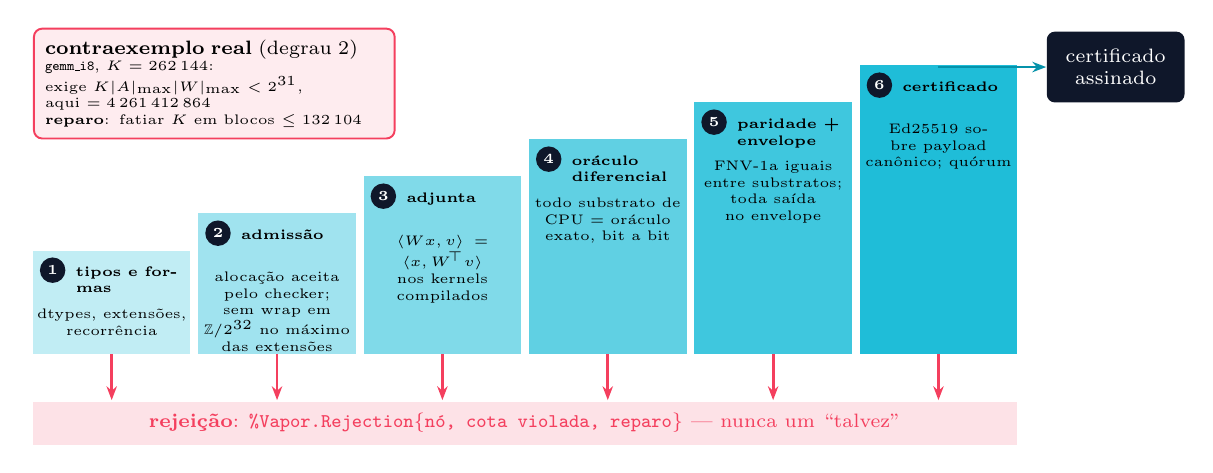
\begin{tikzpicture}
  \foreach \t/\d [count=\ix] in {
      {tipos e formas}/{dtypes, extensões, recorrência},
      {admissão}/{alocação aceita pelo checker; sem wrap em $\mathbb{Z}/2^{32}$ no máximo das extensões},
      {adjunta}/{$\langle Wx,v\rangle = \langle x, W^{\!\top} v\rangle$ nos kernels compilados},
      {oráculo diferencial}/{todo substrato de CPU = oráculo exato, bit a bit},
      {paridade + envelope}/{FNV-1a iguais entre substratos; toda saída no envelope},
      {certificado}/{Ed25519 sobre payload canônico; quórum}} {
    \pgfmathsetmacro{\x}{2.1*(\ix-1)}
    \pgfmathsetmacro{\h}{0.47*\ix+0.85}
    \pgfmathtruncatemacro{\sh}{12+13*\ix}
    \fill[vcyan!\sh] (\x,1.3) rectangle ++(2.0,\h);
    \node[circle,fill=vnavy,text=white,font=\tiny\bfseries,inner sep=1.5pt] at (\x+0.25,1.3+\h-0.25) {\ix};
    \node[font=\tiny\bfseries,anchor=north west,text width=1.55cm,align=left] at (\x+0.42,1.3+\h-0.08) {\t};
    \node[font=\tiny,anchor=north,text width=1.9cm,align=center] at (\x+1.0,1.3+\h-0.62) {\d};
    \draw[rarr] (\x+1.0,1.3) -- (\x+1.0,0.72);
  }
  \node[dark,minimum width=1.75cm,minimum height=0.9cm] (cert) at (13.75,4.95) {certificado\\assinado};
  \draw[carr] (11.5,4.95) -- (cert);
  \fill[vcoral!15] (0,0.15) rectangle (12.5,0.7);
  \node[font=\scriptsize,text=vcoral] at (6.25,0.43) {\textbf{rejeição}: \texttt{\%Vapor.Rejection\{nó, cota violada, reparo\}} --- nunca um ``talvez''};
  \node[badb,text width=4.3cm,align=left,anchor=north west,font=\tiny] at (0.0,5.45) {{\scriptsize\textbf{contraexemplo real} (degrau 2)}\\
    \texttt{gemm\_i8}, $K = 262\,144$:\\
    exige $K|A|_{\max}|W|_{\max} < 2^{31}$,\\ aqui $= 4\,261\,412\,864$\\
    \textbf{reparo}: fatiar $K$ em blocos $\le 132\,104$};
\end{tikzpicture}
\tese{Todo compile termina em \hl{exatamente um} de dois artefatos: um certificado assinado ou um contraexemplo com o reparo. As cotas valem no máximo das extensões e, por monotonia provada, para toda extensão menor.}
\end{frame}

% -------------------------------------------------------------------------
\begin{frame}{Do teorema ao runtime: extração Lean $\to$ Elixir}
\centering
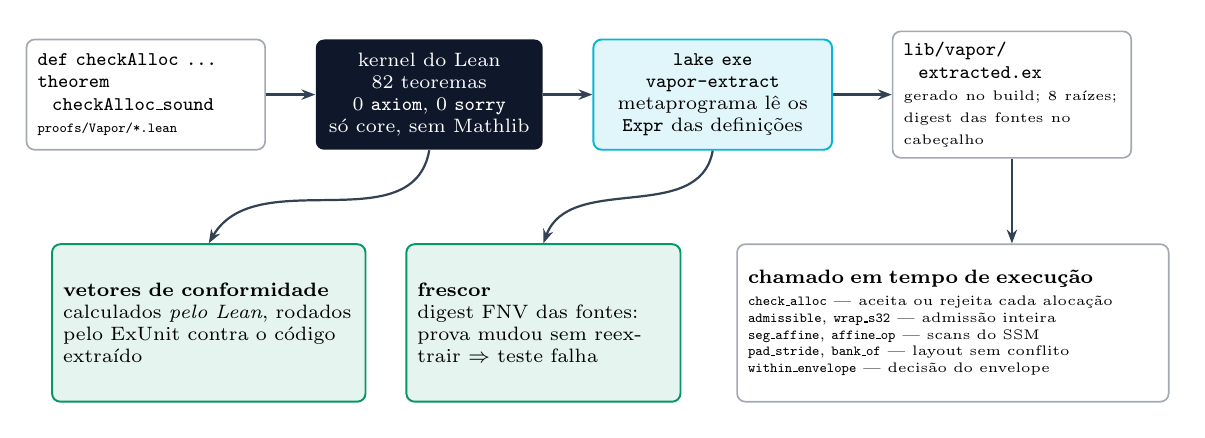
\begin{tikzpicture}[n/.style={box,text width=2.75cm,minimum height=1.4cm}]
  \useasboundingbox (0,-0.1) rectangle (14.6,4.75);
  \node[n,align=left] (l1) at (1.5,3.9) {\texttt{def checkAlloc \ldots}\\\texttt{theorem}\\\texttt{\ \ checkAlloc\_sound}\\{\tiny \texttt{proofs/Vapor/*.lean}}};
  \node[dark,text width=2.6cm,minimum height=1.4cm] (l2) at (5.1,3.9) {kernel do Lean\\82 teoremas\\0 \texttt{axiom}, 0 \texttt{sorry}\\só core, sem Mathlib};
  \node[acc,text width=2.75cm,minimum height=1.4cm] (l3) at (8.7,3.9) {\texttt{lake exe vapor-extract}\\metaprograma lê os \texttt{Expr} das definições};
  \node[n,align=left] (l4) at (12.5,3.9) {\texttt{lib/vapor/}\\\texttt{\ \ extracted.ex}\\{\tiny gerado no build; 8 raízes; digest das fontes no cabeçalho}};
  \draw[arr] (l1)--(l2); \draw[arr] (l2)--(l3); \draw[arr] (l3)--(l4);
  \node[goodb,text width=3.7cm,align=left,minimum height=2.0cm] (v1) at (2.3,1.0) {\textbf{vetores de conformidade}\\calculados \emph{pelo Lean}, rodados pelo ExUnit contra o código extraído};
  \node[goodb,text width=3.2cm,align=left,minimum height=2.0cm] (v2) at (6.55,1.0) {\textbf{frescor}\\digest FNV das fontes: prova mudou sem reextrair $\Rightarrow$ teste falha};
  \node[box,text width=5.2cm,align=left,minimum height=2.0cm,font=\tiny] (u) at (11.75,1.0) {{\scriptsize\textbf{chamado em tempo de execução}}\\[2pt]
    \texttt{check\_alloc} --- aceita ou rejeita cada alocação\\
    \texttt{admissible}, \texttt{wrap\_s32} --- admissão inteira\\
    \texttt{seg\_affine}, \texttt{affine\_op} --- scans do SSM\\
    \texttt{pad\_stride}, \texttt{bank\_of} --- layout sem conflito\\
    \texttt{within\_envelope} --- decisão do envelope};
  \draw[arr] (l2.south) to[out=-100,in=60] (v1.north);
  \draw[arr] (l3.south) to[out=-100,in=70] (v2.north);
  \draw[arr] (l4.south) -- (l4.south |- u.north);
\end{tikzpicture}
\tese{O código que decide no runtime é \hl{o mesmo termo que o Lean verificou}, traduzido mecanicamente no build. Rodar o Lean dentro da BEAM a cada chamada não acrescentaria garantia --- só dependências.}
\end{frame}

% -------------------------------------------------------------------------
\begin{frame}{Árbitro: roofline de três tetos, decisão sem profiling}
\begin{columns}[T]
\begin{column}{0.60\textwidth}
\centering
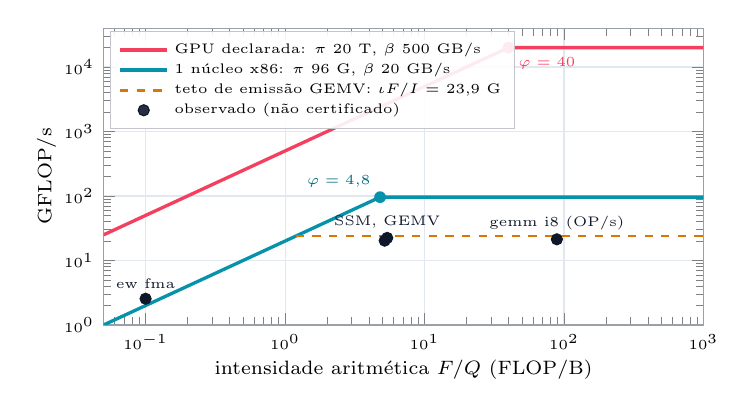
\begin{tikzpicture}
\begin{axis}[
  xmode=log, ymode=log, width=9.2cm, height=5.35cm,
  xmin=0.05, xmax=1000, ymin=1, ymax=40000,
  xlabel={intensidade aritmética $F/Q$ (FLOP/B)}, ylabel={GFLOP/s},
  xlabel style={font=\scriptsize,yshift=3pt}, ylabel style={font=\scriptsize,yshift=-4pt},
  ticklabel style={font=\tiny}, grid=major, grid style={vmist},
  axis line style={vslate!50},
  legend style={font=\tiny,draw=vslate!30,fill=white,fill opacity=0.9,text opacity=1,at={(0.01,0.99)},anchor=north west,row sep=-2pt},
  legend cell align=left]
  \addplot[vcoral,line width=1.2pt] coordinates {(0.05,25) (40,20000) (1000,20000)};
  \addlegendentry{GPU declarada: $\pi$ 20 T, $\beta$ 500 GB/s}
  \addplot[vcyan!80!black,line width=1.2pt] coordinates {(0.05,1) (4.8,96) (1000,96)};
  \addlegendentry{1 núcleo x86: $\pi$ 96 G, $\beta$ 20 GB/s}
  \addplot[vamber,line width=1pt,dashed] coordinates {(1.195,23.9) (1000,23.9)};
  \addlegendentry{teto de emissão GEMV: $\iota F/I$ = 23,9 G}
  \addplot[only marks,mark=*,mark size=2pt,vnavy,
    nodes near coords,point meta=explicit symbolic,nodes near coords style={font=\tiny,anchor=south,text=vnavy}]
    coordinates {(5.18,20.3) [] (5.40,22.4) [SSM, GEMV] (0.10,2.55) [ew fma] (88.9,21.3) [gemm i8 (OP/s)]};
  \addlegendentry{observado (não certificado)}
  \node[circle,fill=vcoral,inner sep=1.5pt] at (axis cs:40,20000) {};
  \node[font=\tiny,text=vcoral,anchor=north west] at (axis cs:40,20000) {$\varphi=40$};
  \node[circle,fill=vcyan!80!black,inner sep=1.5pt] at (axis cs:4.8,96) {};
  \node[font=\tiny,text=vcyan!60!black,anchor=south east] at (axis cs:4.8,96) {$\varphi=4{,}8$};
\end{axis}
\end{tikzpicture}
\end{column}
\begin{column}{0.38\textwidth}
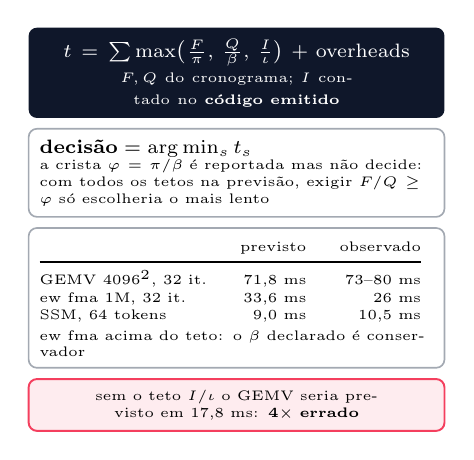
\begin{tikzpicture}
  \node[dark,text width=5.0cm,align=center] (f) {$t=\sum \max\!\big(\tfrac{F}{\pi},\,\tfrac{Q}{\beta},\,\tfrac{I}{\iota}\big)$ + overheads\\[1pt]
    {\tiny $F, Q$ do cronograma; $I$ contado no \textbf{código emitido}}};
  \node[box,text width=5.0cm,align=left,below=0.12cm of f,font=\tiny] (d) {{\scriptsize\textbf{decisão} = $\arg\min_s t_s$}\\
    a crista $\varphi=\pi/\beta$ é reportada mas não decide: com todos os tetos na previsão, exigir $F/Q \ge \varphi$ só escolheria o mais lento};
  \node[box,text width=5.0cm,align=left,below=0.12cm of d,font=\tiny] (r) {\renewcommand{\arraystretch}{1.05}\begin{tabular}{@{}lrr@{}}
      & previsto & observado\\\midrule
      GEMV 4096$^2$, 32 it. & 71,8 ms & 73--80 ms\\
      ew fma 1M, 32 it. & 33,6 ms & 26 ms\\
      SSM, 64 tokens & 9,0 ms & 10,5 ms\\
    \end{tabular}\\[1pt]
    ew fma acima do teto: o $\beta$ declarado é conservador};
  \node[badb,text width=5.0cm,below=0.12cm of r,font=\tiny] {sem o teto $I/\iota$ o GEMV seria previsto em 17,8 ms: \textbf{4$\times$ errado}};
\end{tikzpicture}
\end{column}
\end{columns}
\tese{Trabalho \hl{contado}, hardware \hl{declarado}, tempo \hl{previsto}: a mesma entrada dá a mesma decisão em todo nó, sem aquecimento e sem profiling.}
\end{frame}

% -------------------------------------------------------------------------
\begin{frame}{Certificado, quórum e borda: verificar custa milissegundos}
\centering
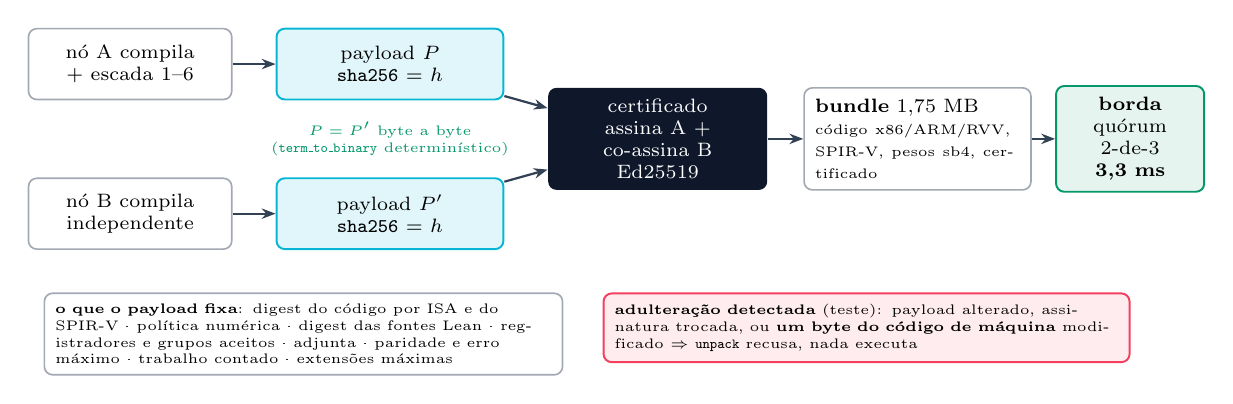
\begin{tikzpicture}[n/.style={box,text width=2.3cm,minimum height=0.9cm}]
  \node[n] (a) at (1.3,4.1) {nó A compila\\+ escada 1--6};
  \node[n] (b) at (1.3,2.2) {nó B compila\\independente};
  \node[acc,text width=2.6cm,minimum height=0.9cm] (pa) at (4.6,4.1) {payload $P$\\\texttt{sha256} = $h$};
  \node[acc,text width=2.6cm,minimum height=0.9cm] (pb) at (4.6,2.2) {payload $P'$\\\texttt{sha256} = $h$};
  \draw[arr] (a)--(pa); \draw[arr] (b)--(pb);
  \node[font=\tiny,text=vgreen,align=center] at (4.6,3.15) {$P = P'$ byte a byte\\(\texttt{term\_to\_binary} determinístico)};
  \node[dark,text width=2.5cm,minimum height=1.2cm] (c) at (8.0,3.15) {certificado\\assina A + co-assina B\\Ed25519};
  \draw[arr] (pa)--(c); \draw[arr] (pb)--(c);
  \node[box,text width=2.6cm,minimum height=1.2cm,align=left] (bd) at (11.3,3.15) {\textbf{bundle} 1,75 MB\\{\tiny código x86/ARM/RVV, SPIR-V, pesos sb4, certificado}};
  \draw[arr] (c)--(bd);
  \node[goodb,text width=1.6cm,minimum height=1.2cm] (e) at (14.0,3.15) {\textbf{borda}\\quórum 2-de-3\\\textbf{3,3 ms}};
  \draw[arr] (bd)--(e);
  % payload
  \node[box,text width=6.3cm,align=left,anchor=north west,font=\tiny] at (0.2,1.2) {\textbf{o que o payload fixa}: digest do código por ISA e do SPIR-V \textperiodcentered{} política numérica
    \textperiodcentered{} digest das fontes Lean \textperiodcentered{} registradores e grupos aceitos \textperiodcentered{} adjunta \textperiodcentered{}
    paridade e erro máximo \textperiodcentered{} trabalho contado \textperiodcentered{} extensões máximas};
  \node[badb,text width=6.4cm,align=left,anchor=north west,font=\tiny] at (7.3,1.2) {\textbf{adulteração detectada} (teste): payload alterado, assinatura trocada, ou \textbf{um byte do código de máquina} modificado $\Rightarrow$ \texttt{unpack} recusa, nada executa};
\end{tikzpicture}
\tese{Certificar custa segundos (10 s no exemplo) e acontece uma vez; verificar custa \hl{3,3 ms} e acontece em cada borda. A borda herda a confiança sem herdar o custo --- nem o toolchain.}
\end{frame}

% =========================================================================
\section{4 · Ecossistema e HPC}
% =========================================================================
\begin{frame}{Do núcleo ao LLM, sem exceções}
\centering
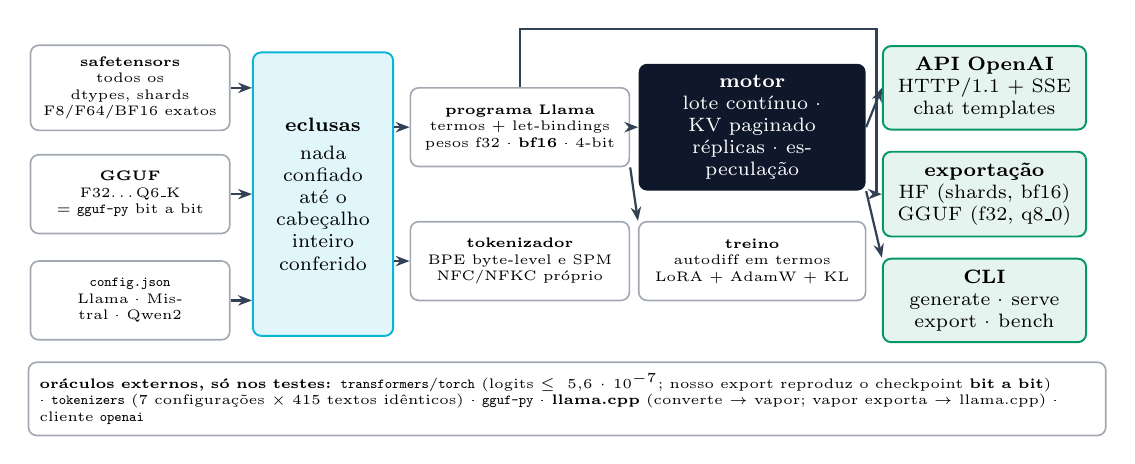
\begin{tikzpicture}[n/.style={box,font=\tiny,text width=2.25cm,minimum height=1.0cm}]
  % entradas
  \node[n] (st) at (1.3,4.3) {\textbf{safetensors}\\todos os dtypes, shards\\F8/F64/BF16 exatos};
  \node[n] (gg) at (1.3,2.95) {\textbf{GGUF}\\F32\ldots Q6\_K\\= \texttt{gguf-py} bit a bit};
  \node[n] (cf) at (1.3,1.6) {\texttt{config.json}\\Llama \textperiodcentered{} Mistral \textperiodcentered{} Qwen2};
  \node[acc,text width=1.5cm,minimum height=3.6cm] (air) at (3.75,2.95) {\textbf{eclusas}\\[2pt]nada confiado\\até o cabeçalho\\inteiro conferido};
  \foreach \s in {st,gg,cf} { \draw[arr] (\s.east) -- (\s.east -| air.west); }
  % programa
  \node[n,text width=2.5cm] (pr) at (6.25,3.8) {\textbf{programa Llama}\\termos + let-bindings\\pesos f32 \textperiodcentered{} \textbf{bf16} \textperiodcentered{} 4-bit};
  \node[n,text width=2.5cm] (tk) at (6.25,2.1) {\textbf{tokenizador}\\BPE byte-level e SPM\\NFC/NFKC próprio};
  \draw[arr] (air.east |- pr) -- (pr); \draw[arr] (air.east |- tk) -- (tk);
  % motor
  \node[dark,text width=2.6cm,minimum height=1.0cm] (en) at (9.2,3.8) {\textbf{motor}\\lote contínuo \textperiodcentered{} KV paginado\\réplicas \textperiodcentered{} especulação};
  \node[n,text width=2.6cm] (tr) at (9.2,2.1) {\textbf{treino}\\autodiff em termos\\LoRA + AdamW + KL};
  \draw[arr] (pr)--(en); \draw[arr] (pr.south east) -- (tr.north west);
  % saídas
  \node[goodb,text width=2.3cm,minimum height=1.0cm] (api) at (12.15,4.3) {\textbf{API OpenAI}\\HTTP/1.1 + SSE\\chat templates};
  \node[goodb,text width=2.3cm,minimum height=1.0cm] (ex) at (12.15,2.95) {\textbf{exportação}\\HF (shards, bf16)\\GGUF (f32, q8\_0)};
  \node[goodb,text width=2.3cm,minimum height=1.0cm] (cli) at (12.15,1.6) {\textbf{CLI}\\generate \textperiodcentered{} serve\\export \textperiodcentered{} bench};
  \draw[arr] (en.east) -- (api.west); \draw[arr] (pr.north) |- (10.78,5.05) |- (ex.west);
  \draw[arr] (en.south east) -- (cli.north west);
  % oráculos
  \node[box,text width=13.4cm,align=left,font=\tiny] at (6.85,0.35) {\textbf{oráculos externos, só nos testes:} \texttt{transformers}/\texttt{torch} (logits $\le 5{,}6\cdot10^{-7}$; nosso export reproduz o checkpoint \textbf{bit a bit})
    \textperiodcentered{} \texttt{tokenizers} (7 configurações $\times$ 415 textos idênticos) \textperiodcentered{} \texttt{gguf-py} \textperiodcentered{} \textbf{llama.cpp} (converte $\to$ vapor; vapor exporta $\to$ llama.cpp) \textperiodcentered{} cliente \texttt{openai}};
\end{tikzpicture}
\tese{Nenhuma camada nova pediu exceção às garantias: os modelos são \hl{programas da mesma álgebra} --- mesmos kernels, mesma escada, mesmos bits em CPU, RISC-V e GPU.}
\end{frame}

% -------------------------------------------------------------------------
\begin{frame}{HPC sem trocar bits}
\centering
\scriptsize
\renewcommand{\arraystretch}{1.13}
\begin{tabular}{@{}p{2.55cm}p{6.1cm}p{4.9cm}@{}}
\toprule
\textbf{forma} & \textbf{onde} & \textbf{invariante testado}\\
\midrule
SIMD & AVX2 \textperiodcentered{} \textbf{AVX-512} (EVEX, 32 zmm, cauda mascarada) \textperiodcentered{} NEON \textperiodcentered{} RVV 128--512 \textperiodcentered{} SPIR-V & mesmos bits que o oráculo\\
ILP & GEMV com 4/2/1 linhas por iteração, escolhido pelo alocador & idem\\
threads & pool no worker; descritor de partição por chamada; decode dividido por cabeça KV & 1 = 2 = 3 threads\\
lote contínuo & decode + pedaços de prefill no mesmo passo & sozinho = em lote, qualquer fatiamento\\
KV paginado & tabela de blocos, páginas reservadas na admissão & paginado = contíguo\\
réplicas & uma compilação, \textbf{mesmas páginas de pesos}, menor fila & qualquer réplica; falha isolada\\
banda & GEMV \emph{weight-stationary}; pesos \textbf{bf16} residentes alargados no kernel & bf16 = f32 sobre pesos arredondados\\
especulação & rascunho propõe, alvo verifica $k{+}1$ linhas num passo & saída = alvo sozinho\\
GPU & SPIR-V de todo operador de modelo & fabric = oráculo (modelo inteiro)\\
concorrência BEAM & processo por conexão, motor \texttt{GenServer}, SSE; worker morto $\to$ \texttt{:error}, sessão reaberta & --- \\
\bottomrule
\end{tabular}
\tese{A soma nunca é reassociada: o paralelismo vem de \hl{linhas, sequências, réplicas e cabeças independentes}. Por isso cada forma de HPC entra sem custar a garantia central.}
\end{frame}

% -------------------------------------------------------------------------
\begin{frame}{Medido: AVX-512, bf16, threads e o motor}
\begin{columns}[T]
\begin{column}{0.52\textwidth}
\centering
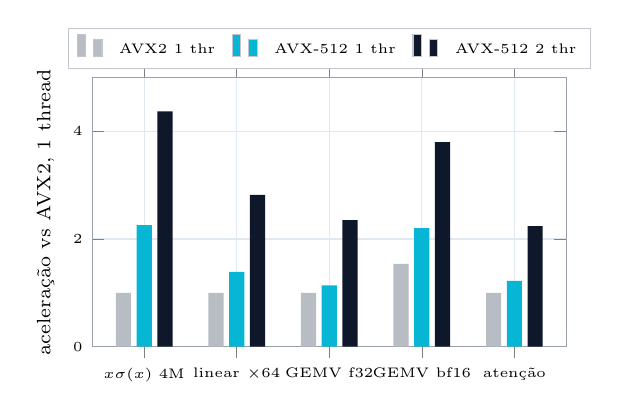
\begin{tikzpicture}
\begin{axis}[
  ybar, width=7.6cm, height=5.0cm, bar width=5.5pt,
  symbolic x coords={silu,linear,GEMVf32,GEMVbf16,atencao},
  xticklabels={$x\sigma(x)$ 4M, linear $\times$64, GEMV f32, GEMV bf16, atenção},
  xtick=data, ymin=0, ymax=5,
  ylabel={aceleração vs AVX2, 1 thread}, ylabel style={font=\scriptsize},
  ticklabel style={font=\tiny}, grid=major, grid style={vmist}, axis line style={vslate!50},
  legend style={font=\tiny,draw=vslate!30,at={(0.5,1.03)},anchor=south,legend columns=3,column sep=4pt},
  legend cell align=left, enlarge x limits=0.14]
  \addplot[fill=vslate!35,draw=none] coordinates {(silu,1) (linear,1) (GEMVf32,1) (GEMVbf16,1.54) (atencao,1)};
  \addplot[fill=vcyan,draw=none] coordinates {(silu,2.26) (linear,1.39) (GEMVf32,1.14) (GEMVbf16,2.20) (atencao,1.22)};
  \addplot[fill=vnavy,draw=none] coordinates {(silu,4.37) (linear,2.82) (GEMVf32,2.35) (GEMVbf16,3.80) (atencao,2.24)};
  \legend{AVX2 1 thr, AVX-512 1 thr, AVX-512 2 thr}
\end{axis}
\end{tikzpicture}
\fonte{GEMV 2048$^2$; bf16 relativo ao GEMV f32 AVX2. Banda medida: 53 GB/s. \texttt{docs/bench/BENCH.md}, 2026-10-01.}
\end{column}
\begin{column}{0.46\textwidth}
\centering
\scriptsize
\renewcommand{\arraystretch}{1.12}
\begin{tabular}{@{}lrr@{}}
\toprule
\textbf{motor} (Llama 256, vocab 32k) & seq. & tokens/s\\
\midrule
AVX2, 1 thread & 8 & 895\\
AVX2, 2 threads & 8 & 1\,477\\
2 réplicas $\times$ 1 thread & 8 & 1\,555\\
AVX-512, 2 threads, f32 & 1 & 403\\
AVX-512, 2 threads, \textbf{bf16} & 1 & \textbf{588}\\
prefill, 256 tokens & --- & $\sim$5\,500\\
\bottomrule
\end{tabular}\\[6pt]
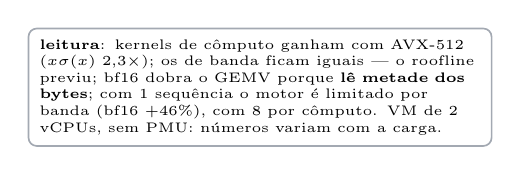
\begin{tikzpicture}
  \node[box,text width=5.6cm,align=left,font=\tiny] {\textbf{leitura}: kernels de cômputo ganham com AVX-512 ($x\sigma(x)$ 2,3$\times$); os de banda ficam
    iguais --- o roofline previu; bf16 dobra o GEMV porque \textbf{lê metade dos bytes}; com 1 sequência o motor é limitado por banda
    (bf16 +46\%), com 8 por cômputo. VM de 2 vCPUs, sem PMU: números variam com a carga.};
\end{tikzpicture}
\end{column}
\end{columns}
\tese{Os ganhos vêm de \hl{onde o roofline diz que estão} --- largura vetorial onde há cômputo, bytes a menos onde há banda --- e nenhum deles muda um bit da saída.}
\end{frame}

% -------------------------------------------------------------------------
\begin{frame}{Interoperabilidade conferida por terceiros}
\centering
\scriptsize
\renewcommand{\arraystretch}{1.15}
\begin{tabular}{@{}p{4.3cm}p{3.6cm}p{5.6cm}@{}}
\toprule
\textbf{caminho} & \textbf{juiz} & \textbf{resultado}\\
\midrule
checkpoint HF $\to$ vapor & \texttt{transformers} f32 & logits $\le 5{,}6\cdot10^{-7}$ rel.; greedy idêntico (5 variantes)\\
vapor $\to$ diretório HF $\to$ transformers & \texttt{transformers} & logits do checkpoint original \textbf{bit a bit}; bf16 $\le 10^{-5}$\\
safetensors de todo dtype & \texttt{torch}, \texttt{numpy} & F8 (os 256 padrões de cada formato), F64, F16, inteiros: \textbf{bit a bit}\\
f32 $\to$ BF16/F16 na escrita & \texttt{torch} & 20\,000 padrões (empates, subnormais, overflow) \textbf{bit a bit}\\
HF $\to$ \texttt{convert\_hf\_to\_gguf.py} $\to$ vapor & \texttt{transformers} & f32 $5{,}6\cdot10^{-7}$ rel.; q8\_0 dentro da quantização\\
desquantização GGUF (11 tipos), Q8\_0 & \texttt{gguf-py} & \textbf{bit a bit}\\
vapor $\to$ GGUF $\to$ llama.cpp & \texttt{libllama} & mesma tokenização; logits f32 $\le 10^{-4}$, q8\_0 $\le 5\%$\\
tokenizador (4 vocabulários reais) & \texttt{tokenizers} & 184 vetores HF + 2\,905 textos: idênticos\\
servidor & cliente \texttt{openai} & completions e chat, com e sem streaming\\
\bottomrule
\end{tabular}
\tese{Um formato só está suportado quando \hl{a ferramenta de referência concorda} --- lendo o que ela escreve e escrevendo o que ela lê. Os juízes rodam só nos testes; o produto continua \texttt{deps: []}.}
\end{frame}

% =========================================================================
\section{5 · Agentes, RAG e ZK}
% =========================================================================
\begin{frame}{Fronteira: as famílias abertas como contrações exatas}
\centering
\scriptsize
\renewcommand{\arraystretch}{1.15}
\begin{tabular}{@{}p{2.4cm}p{4.9cm}p{6.3cm}@{}}
\toprule
\textbf{família} & \textbf{o que exige} & \textbf{como entrou (sem operador aproximado)}\\
\midrule
Qwen3 & normas RMS por cabeça em q/k & \texttt{linear} com matrizes de seleção 0/1\\
Qwen3-MoE, Mixtral & roteador top-$k$, especialistas & posto por contagem + \texttt{sel}; soma em ordem fixa de especialista\\
Gemma 3 & GeGLU (tanh), normas $(1{+}w)$ e sanduíche, RoPE local/global & novas funções canônicas \texttt{tanh}, \texttt{gelu\_tanh}; escala de atenção explícita\\
DeepSeek-V3 & MLA, MoE por grupos (sigmoide), YaRN & MLA como layout de cabeças; grupos por seleção exata; tabelas \textbf{corretamente arredondadas}\\
\midrule
\multicolumn{3}{@{}l}{\textbf{juiz}: \texttt{transformers} 5.18 --- logits $\le 8\cdot10^{-7}$ rel. em 8 variantes; mesmos bits em AVX2, AVX-512, RVV, QEMU, Vulkan}\\
\multicolumn{3}{@{}l}{especialistas \emph{não escolhidos} envenenados com NaN/$\infty$: \textbf{nenhum bit muda}; prefill = decode passo a passo}\\
\bottomrule
\end{tabular}\\[6pt]
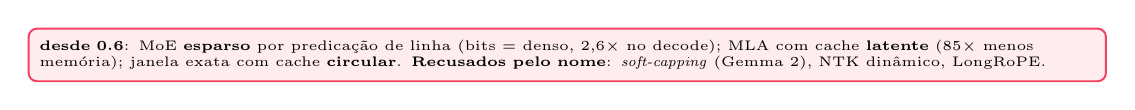
\begin{tikzpicture}
  \node[badb,text width=13.4cm,align=left,font=\tiny] {\textbf{desde 0.6}: MoE \textbf{esparso} por predicação de linha (bits = denso, 2{,}6$\times$ no decode); MLA com cache \textbf{latente} (85$\times$ menos memória); janela exata com cache \textbf{circular}. \textbf{Recusados pelo nome}: \emph{soft-capping} (Gemma 2), NTK dinâmico, LongRoPE.};
\end{tikzpicture}
\tese{Cada peça nova das arquiteturas de fronteira virou \hl{uma contração exata da mesma álgebra} --- por isso herdou, sem exceção, os mesmos bits em todo substrato.}
\end{frame}

% -------------------------------------------------------------------------
\begin{frame}{Agentes imutáveis: a execução é um objeto de prova}
\centering
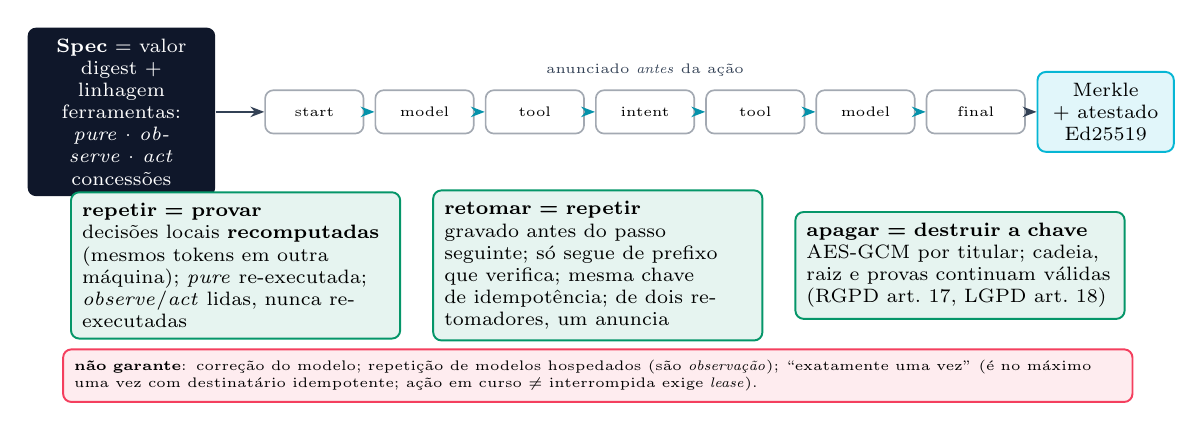
\begin{tikzpicture}[ev/.style={box,font=\tiny,minimum width=1.25cm,minimum height=0.55cm}]
  \node[dark,text width=2.1cm] (sp) at (0.55,3.3) {\textbf{Spec} = valor\\digest + linhagem\\ferramentas: \emph{pure} \textperiodcentered{} \emph{observe} \textperiodcentered{} \emph{act}\\concessões};
  \foreach \k [count=\ix] in {start,model,tool,intent,tool,model,final} {
    \node[ev] (e\ix) at (1.6+1.4*\ix,3.3) {\k};
  }
  \draw[arr] (sp) -- (e1);
  \foreach \ix [evaluate=\ix as \j using int(\ix+1)] in {1,...,6} { \draw[carr] (e\ix) -- (e\j); }
  \node[lbl,above=0.05cm of e4] {anunciado \emph{antes} da ação};
  \node[acc,text width=1.45cm] (at) at (13.05,3.3) {Merkle\\+ atestado\\Ed25519};
  \draw[arr] (e7) -- (at);
  \node[goodb,text width=3.9cm,minimum height=1.35cm,align=left] at (2.0,1.35) {\textbf{repetir = provar}\\decisões locais \textbf{recomputadas} (mesmos tokens em outra máquina); \emph{pure} re-executada; \emph{observe}/\emph{act} lidas, nunca re-executadas};
  \node[goodb,text width=3.9cm,minimum height=1.35cm,align=left] at (6.6,1.35) {\textbf{retomar = repetir}\\gravado antes do passo seguinte; só segue de prefixo que verifica; mesma chave de idempotência; de dois retomadores, um anuncia};
  \node[goodb,text width=3.9cm,minimum height=1.35cm,align=left] at (11.2,1.35) {\textbf{apagar = destruir a chave}\\AES-GCM por titular; cadeia, raiz e provas continuam válidas (RGPD art.~17, LGPD art.~18)};
  \node[badb,text width=13.3cm,align=left,font=\tiny] at (6.6,-0.05) {\textbf{não garante}: correção do modelo; repetição de modelos hospedados (são \emph{observação}); “exatamente uma vez” (é no máximo uma vez com destinatário idempotente; ação em curso $\neq$ interrompida exige \emph{lease}).};
\end{tikzpicture}
\tese{O laço de agente é \emph{commodity}; o que só o vapor tem é determinismo --- e com ele um agente deixa de produzir \hl{logs} e passa a produzir \hl{provas}.}
\end{frame}

% -------------------------------------------------------------------------
\begin{frame}{Por construção --- e o ecossistema Elixir}
\begin{columns}[T]
\begin{column}{0.53\textwidth}
\scriptsize
\begin{itemize}\setlength\itemsep{3pt}
\item \textbf{JSON Schema e tool calls} como gramática de bytes sobre a trie do vocabulário: válidos \hl{sem retry}; 0--50 ms/token no vocabulário de 151\,936
\item \textbf{nenhum beco sem saída}: o teste de propriedade achou 3 (escape no \texttt{maxLength}, surrogate solto, UTF-8 malformado) --- corrigidos
\item \textbf{RAG}: corpus = raiz Merkle; BM25 e densos determinísticos; recibo re-verificável; dentro de \texttt{<quote>} só \hl{substrings literais} da fonte
\item \textbf{Jinja hermético}: 240 renderizações de 20 templates reais = \texttt{jinja2} byte a byte
\item \textbf{recibo} \texttt{x-vapor-receipt}: quem tem os pesos re-deriva a resposta
\end{itemize}
\end{column}
\begin{column}{0.45\textwidth}
\centering
\scriptsize
\renewcommand{\arraystretch}{1.1}
\begin{tabular}{@{}>{\raggedright\arraybackslash}p{2.25cm}>{\raggedright\arraybackslash}p{3.7cm}@{}}
\toprule
\textbf{Elixir} & \textbf{veredito}\\
\midrule
Plug, Phoenix & \mbox{\ok} \texttt{Vapor.Plug} (Bandit, testado)\\
Nx & \mbox{\ok} compilador \texttt{defn} certificado (fragmento)\\
Livebook & \mbox{\ok} passeio executado como teste\\
Ecto, Oban, LiveView & \emph{behaviour} \texttt{Store}, \texttt{on\_event}, cancelamento\\
Broadway, EMQX & ingestão / transporte de eventos\\
Nerves & viável (workers estáticos); sem placa\\
AtomVM, Membrane, Riak & \mbox{\no} com motivo\\
\bottomrule
\end{tabular}
\end{column}
\end{columns}
\tese{O núcleo continua \texttt{deps: []}: o ecossistema entra por \hl{pontos de extensão}, e integrar de verdade revelou defeitos que a descrição escondia (cliente desconectado gerando, \emph{code path} podado).}
\end{frame}

% -------------------------------------------------------------------------
\begin{frame}{ZK e FHE: fato, analogia, construído}
\centering
\scriptsize
\renewcommand{\arraystretch}{1.12}
\begin{tabular}{@{}>{\raggedright\arraybackslash}p{4.1cm}>{\raggedright\arraybackslash}p{4.3cm}>{\raggedright\arraybackslash}p{5.0cm}@{}}
\toprule
\textbf{proposta} & \textbf{escrutínio} & \textbf{feito e testado}\\
\midrule
RVV para zkVMs (SP1, RISC Zero) & \leavevmode\bad{premissa falsa}: zkVMs são RV32IM & testemunha pelos kernels certificados, sem zkVM\\
aritmetizar \texttt{add}/\texttt{mul}/\texttt{fma} & \leavevmode f32 \bad{não} é aritmética de corpo & int8 $\to$ R1CS: 16$\to$8$\to$3 = 311 restrições (144 de faixa da entrada); Groth16 ok, forjado rejeitado\\
verificador on-chain ``$<$200k gás'' & depende do verificador & \leavevmode\hl{medido}: 209\,922 gás (execução), 3 entradas públicas\\
Lean ``elimina 100\% dos riscos'' & exagero: setup, provador, pesos certos & lema provado: $2KAB<p \Rightarrow$ máquina = $\mathbb{Z}$ = $\mathbb{F}_p$\\
NTT para FHE e STARK & núcleo comum, vale o kernel & referência exata em 4 corpos, cíclica e negacíclica\\
Wilkinson = orçamento de ruído & \leavevmode\bad{analogia}: ruído CKKS é aleatório & ---\\
ativações por Chebyshev & \leavevmode\texttt{Canon} \bad{não} é polinomial puro & erro \hl{provado} em racionais (sigmoide gr.~15: $1{,}388\cdot10^{-3}$)\\
CKKS/BFV na álgebra; zkFHE 70B & cripto sem auditoria; pesquisa & recusado (OpenFHE, Lattigo existem)\\
\bottomrule
\end{tabular}
\tese{Com pesos públicos, o \hl{recibo determinístico} já verifica por reexecução: ZK só se paga por \hl{privacidade} ou \hl{verificação sucinta} --- e então o fragmento inteiro, com a ponte provada em Lean, é o caminho barato.}
\end{frame}

% =========================================================================
\section{6 · Para quem}
% =========================================================================
\begin{frame}{Pilha tradicional $\times$ vapor --- inclusive onde o vapor perde}
\centering
\scriptsize
\renewcommand{\arraystretch}{1.08}
\begin{tabular}{@{}p{3.0cm}p{5.2cm}p{5.5cm}@{}}
\toprule
& \textbf{PyTorch / CUDA / vLLM} & \textbf{vapor}\\
\midrule
Instalação & 3,0 GB de wheels (torch 2.14 + CUDA) & \win 1,8 MB no núcleo; 8,7 MB com as 13 rodadas (+ runtime Erlang)\\
Geração de código & LLVM, NVCC, Triton, \texttt{ptxas}: C++ na base de confiança & \win codificadores puros em Elixir $\to$ bits, juiz externo em teste\\
Falha do driver & no mesmo processo: derruba o serviço & \win processo separado, erro tipado, failover\\
Determinismo & modo determinístico parcial; muda com GPU e versão & \win \texttt{:canonical} bit-idêntico em x86, ARM, RVV e GPU\\
Garantia formal & nenhuma sobre o código gerado & \win checker, admissão, envelope provados e extraídos\\
Artefato de implantação & imagem de container & \win bundle assinado, quórum, verificação em ms\\
Previsão de desempenho & profiling e autotuning empíricos & \win contada e declarada: mesma decisão em todo nó\\
RISC-V RVV & fora do caminho principal de otimização & \win alvo de primeira classe, agnóstico a VLEN\\
\midrule
Cobertura de operadores & \lose\textbf{milhares} de ops, qualquer arquitetura & 8 famílias (Llama\ldots{} DeepSeek-V3), GEMM i8, SSM\\
Desempenho de pico & \lose tensor cores, kernels ajustados à mão & AVX-512, threads; coopmat não executado\\
Treino e ecossistema & \lose autograd completo, distribuído, comunidade & autodiff + LoRA (modelos pequenos)\\
\bottomrule
\end{tabular}\\[3pt]
{\tiny \win vantagem \quad \lose vantagem do lado oposto}
\tese{Não é um substituto do PyTorch: é \hl{outro ponto do espaço de projeto} --- menos cobertura e menos pico, em troca de garantias que a pilha tradicional não tem como oferecer.}
\end{frame}

% -------------------------------------------------------------------------
\begin{frame}{Para quem isso muda o jogo hoje}
\centering
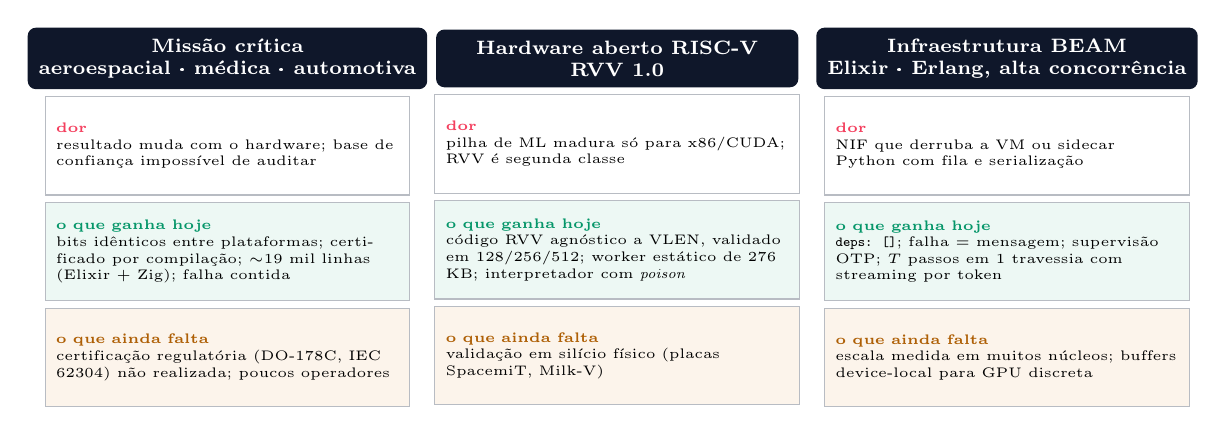
\begin{tikzpicture}[hd/.style={dark,minimum width=4.6cm,minimum height=0.7cm,font=\scriptsize\bfseries},
                    cell/.style={draw=vslate!35,fill=white,text width=4.35cm,align=left,font=\tiny,inner sep=4pt,minimum height=1.25cm}]
  \foreach \h/\p/\g/\f [count=\ix] in {
    {Missão crítica\\aeroespacial \textperiodcentered{} médica \textperiodcentered{} automotiva}/
      {resultado muda com o hardware; base de confiança impossível de auditar}/
      {bits idênticos entre plataformas; certificado por compilação; $\sim$19 mil linhas (Elixir + Zig); falha contida}/
      {certificação regulatória (DO-178C, IEC 62304) não realizada; poucos operadores},
    {Hardware aberto RISC-V\\RVV 1.0}/
      {pilha de ML madura só para x86/CUDA; RVV é segunda classe}/
      {código RVV agnóstico a VLEN, validado em 128/256/512; worker estático de 276 KB; interpretador com \emph{poison}}/
      {validação em silício físico (placas SpacemiT, Milk-V)},
    {Infraestrutura BEAM\\Elixir \textperiodcentered{} Erlang, alta concorrência}/
      {NIF que derruba a VM ou sidecar Python com fila e serialização}/
      {\texttt{deps: []}; falha = mensagem; supervisão OTP; $T$ passos em 1 travessia com streaming por token}/
      {escala medida em muitos núcleos; buffers device-local para GPU discreta}} {
    \pgfmathsetmacro{\x}{4.95*(\ix-1)}
    \node[hd,align=center] (h\ix) at (\x+2.3,4.9) {\h};
    \node[cell,anchor=north] (p\ix) at ($(h\ix.south)+(0,-0.08)$) {\textcolor{vcoral}{\textbf{dor}}\\ \p};
    \node[cell,anchor=north,fill=vgreen!7] (g\ix) at ($(p\ix.south)+(0,-0.08)$) {\textcolor{vgreen}{\textbf{o que ganha hoje}}\\ \g};
    \node[cell,anchor=north,fill=vamber!8] (f\ix) at ($(g\ix.south)+(0,-0.08)$) {\textcolor{vamber!80!black}{\textbf{o que ainda falta}}\\ \f};
  }
\end{tikzpicture}
\tese{Muda o jogo onde \hl{reprodutibilidade, auditabilidade e tolerância a falhas} valem mais que os últimos 10\% de throughput --- e diz com clareza o que ainda não entrega.}
\end{frame}

\begin{frame}{Rodada 0.6: fronteira, imagem e áudio --- sem perder os bits}
\centering
\tiny
\renewcommand{\arraystretch}{1.18}
\begin{tabular}{@{}p{3.0cm}p{6.0cm}p{4.6cm}@{}}
\toprule
\textbf{recurso} & \textbf{como (primeiros princípios)} & \textbf{evidência}\\
\midrule
MoE esparso & predicação por linha no GEMV: não ler pesos que ninguém escolheu & bits = denso; 2{,}6$\times$ no decode\\
MLA latente & outro programa (absorção), escolhido pelo operador & 85$\times$ menos cache; = \texttt{transformers}\\
janela + anel & anel na \emph{tabela de blocos}: ordem lógica intacta, $R=\lceil (w{+}T{-}1)/p\rceil$ & limite justo (controle); 7{,}9$\times$ seqs.\\
Mamba & a recorrência é a definição; estado realimentado no worker & = \texttt{transformers}; custo/token constante\\
árvore especulativa & ramos em \emph{slots} sobre páginas compartilhadas; o vencedor herda as páginas & saída = gulosa; 6 tokens/passo\\
tensor paralelo & coluna + all-gather (linha + all-reduce muda 81\% dos bits) & bits = 1 worker\\
conv / VAE / DiT & im2col = \texttt{gather} + \texttt{sel} + \texttt{reshape} + GEMV: nenhum kernel novo & $\le 9\cdot10^{-7}$ vs. torch/diffusers\\
Whisper & encoder + decoder como \emph{partes} do contrato; K/V cruzados 1$\times$ & gulosa = \texttt{transformers}\\
$\div$ IEEE, Higham & Markstein + Dekker sem FMA (semântica v2); Higham em Lean & 0 erros em $5\cdot10^{7}$\\
log de transparência & RFC 9162 + C2SP, testemunhas, verificação no navegador & 196 sondas do transparency-dev\\
\bottomrule
\end{tabular}\\[3pt]
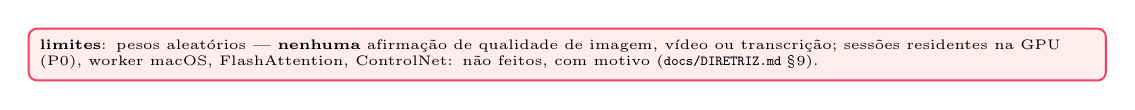
\begin{tikzpicture}
  \node[badb,text width=13.4cm,align=left,font=\tiny] {\textbf{limites}: pesos aleatórios --- \textbf{nenhuma} afirmação de qualidade de imagem, vídeo ou transcrição; sessões residentes na GPU (P0), worker macOS, FlashAttention, ControlNet: não feitos, com motivo (\texttt{docs/DIRETRIZ.md} §9).};
\end{tikzpicture}
\tese{Cada truque de serviço que costuma \hl{trocar reprodutibilidade por velocidade} entrou aqui sem essa troca --- e com o seu custo medido ao lado.}
\end{frame}

\begin{frame}{Rodada 0.7: o escaneado e o LM que sabe se calar}
\centering
\tiny
\renewcommand{\arraystretch}{1.18}
\begin{tabular}{@{}p{3.0cm}p{6.0cm}p{4.6cm}@{}}
\toprule
\textbf{recurso} & \textbf{como (primeiros princípios)} & \textbf{evidência (com controle)}\\
\midrule
CCITT G3/G4, LZW & T.4/T.6 em Elixir, a máquina de estados do Xpdf & 42 fluxos = libtiff bit a bit\\
ordem de leitura & XY-cut: a \emph{calha} corta antes do vão; limiares da própria região & 8 páginas: CER 1{,}3\% (sem ordem: 53\%; Tesseract 1{,}6\%)\\
feixe + LM & 5-gramas Witten--Bell; só escolhe entre o que os quadros acham plausível & retidas 6{,}5\% $\to$ 4{,}4\%; embaralhado: nenhum ganho\\
abstenção & acima de 8 bits/caractere a linha não é língua: o modelo se cala & aleatórias: 0/30 mudadas (sem guarda: 27)\\
\texttt{pattern} / \texttt{format} & regex ECMA-262 $\to$ autômato de bytes UTF-8 com escapes JSON & = \texttt{re} do Python em 7\,240 cadeias\\
fusão em disco & um tensor por vez, mesmos kernels, cabeçalho antes dos dados & mesmos bytes; 4 MB $\times$ 83 MB\\
\bottomrule
\end{tabular}\\[3pt]
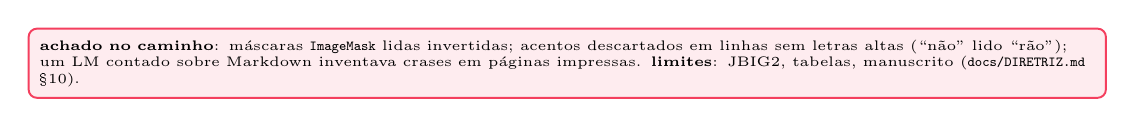
\begin{tikzpicture}
  \node[badb,text width=13.4cm,align=left,font=\tiny] {\textbf{achado no caminho}: máscaras \texttt{ImageMask} lidas invertidas; acentos descartados em linhas sem letras altas (``não'' lido ``rão''); um LM contado sobre Markdown inventava crases em páginas impressas. \textbf{limites}: JBIG2, tabelas, manuscrito (\texttt{docs/DIRETRIZ.md} §10).};
\end{tikzpicture}
\tese{Um modelo de língua é o exemplo clássico de \hl{ruído plausível}: aqui ele só entra com o controle que mostra onde ele \emph{não} deve falar.}
\end{frame}

% =========================================================================
\section{7 · Rodadas}
% =========================================================================
\begin{frame}{De 0.8 a 0.14: um domínio por vez --- e então a bancada aberta}
\centering
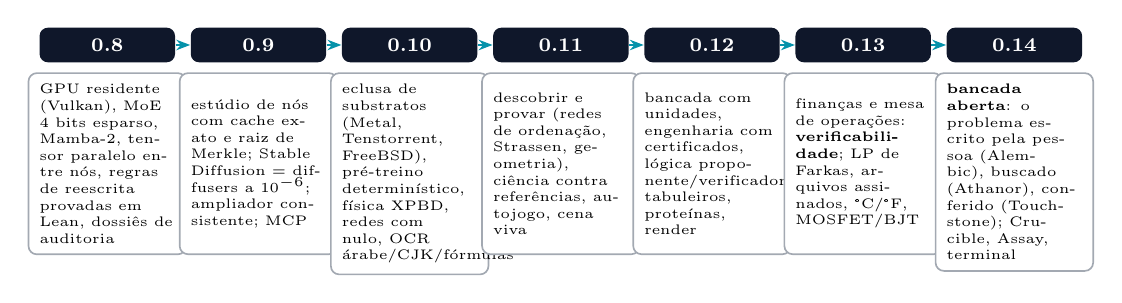
\begin{tikzpicture}[r/.style={box,text width=1.72cm,minimum height=2.3cm,align=left,anchor=north,font=\tiny},
                    v/.style={dark,font=\scriptsize\bfseries,minimum width=1.72cm}]
  \foreach \v/\t [count=\ix] in {
    0.8/{GPU residente (Vulkan), MoE 4 bits esparso, Mamba-2, tensor paralelo entre nós, regras de reescrita provadas em Lean, dossiês de auditoria},
    0.9/{estúdio de nós com cache exato e raiz de Merkle; Stable Diffusion = diffusers a $10^{-6}$; ampliador consistente; MCP},
    0.10/{eclusa de substratos (Metal, Tenstorrent, FreeBSD), pré-treino determinístico, física XPBD, redes com nulo, OCR árabe/CJK/fórmulas},
    0.11/{descobrir e provar (redes de ordenação, Strassen, geometria), ciência contra referências, autojogo, cena viva},
    0.12/{bancada com unidades, engenharia com certificados, lógica proponente/verificador, tabuleiros, proteínas, render},
    0.13/{finanças e mesa de operações: \textbf{verificabilidade}; LP de Farkas, arquivos assinados, °C/°F, MOSFET/BJT},
    0.14/{\textbf{bancada aberta}: o problema escrito pela pessoa (Alembic), buscado (Athanor), conferido (Touchstone); Crucible, Assay, terminal}} {
    \node[v] (h\ix) at (1.92*\ix,0) {\v};
    \node[r] at ($(h\ix.south)+(0,-0.12)$) {\t};
  }
  \foreach \ix [evaluate=\ix as \j using int(\ix+1)] in {1,...,6} \draw[carr] (h\ix) -- (h\j);
\end{tikzpicture}\\[6pt]
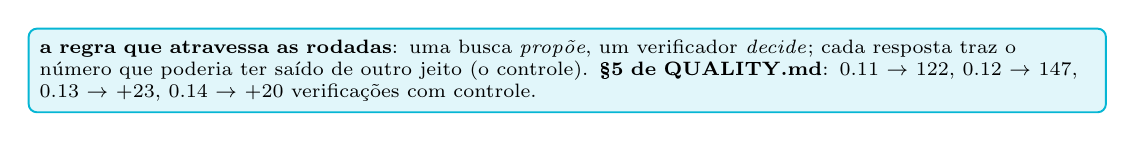
\begin{tikzpicture}
  \node[acc,text width=13.4cm,align=left,font=\scriptsize] {\textbf{a regra que atravessa as rodadas}: uma busca \emph{propõe}, um verificador \emph{decide}; cada resposta traz o número que poderia ter saído de outro jeito (o controle). \textbf{§5 de QUALITY.md}: 0.11 $\to$ 122, 0.12 $\to$ 147, 0.13 $\to$ +23, 0.14 $\to$ +20 verificações com controle.};
\end{tikzpicture}
\tese{A amplitude cresceu sem que o núcleo mudasse de natureza: \hl{cada domínio novo entra pela mesma porta --- a do certificado}.}
\end{frame}

\begin{frame}{0.13: finanças --- verificabilidade, não velocidade}
\centering\tiny
\renewcommand{\arraystretch}{1.16}
\begin{tabular}{@{}p{2.6cm}p{5.6cm}p{5.4cm}@{}}
\toprule
\textbf{tarefa} & \textbf{o que entra (texto da mesa)} & \textbf{o certificado que sai}\\
\midrule
calendários, dinheiro & \texttt{du 2025-01-02 2026-01-02}, \texttt{allocate 100.00 1 1 1} & feriados por regra (cômputo) \hl{= QuantLib dia a dia, 1990--2078}; rateio que soma exatamente\\
curvas & DI1, LTN, NTN-F, depósitos, swaps & todo instrumento reprecificado ($4{,}5\cdot10^{-16}$); forwards negativos apontados\\
opções & \texttt{price/iv/american/heston/smile} & paridade; gregas $\times$ dif. finitas; limites de não arbitragem \emph{antes}; $g(k)\ge0$ de Durrleman; \hl{= QuantLib} ($10^{-9}$--$10^{-12}$)\\
Monte Carlo & S, K, T, r, $\sigma$, trajetórias, barreira & bits = oráculo = 2 threads; IC de 99\% $\times$ forma fechada\\
risco & P\&L e método de VaR & Kupiec, Christoffersen, Basileia; \hl{tamanho e poder do teste medidos}\\
backtest & dados, varredura, sinal causal, custo & \hl{quatro portões}: prefixo, DSR, PBO, Reality Check\\
arbitragem & estados / calls / câmbio & \hl{um portfólio ou preços de estado}, em $\mathbb{Q}$\\
livro de ofertas & \texttt{buy 100 @ 101.25 gtc owner=a} & diário SHA-256 + Merkle; \hl{juiz ingênuo}; ITCH; FIX\\
\bottomrule
\end{tabular}\\[4pt]
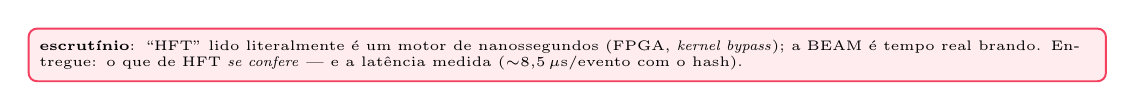
\begin{tikzpicture}
  \node[badb,text width=13.4cm,align=left,font=\tiny] {\textbf{escrutínio}: ``HFT'' lido literalmente é um motor de nanossegundos (FPGA, \emph{kernel bypass}); a BEAM é tempo real brando. Entregue: o que de HFT \emph{se confere} --- e a latência medida (${\sim}8{,}5\,\mu$s/evento com o hash).};
\end{tikzpicture}
\tese{Um preço que muda de máquina para máquina, um backtest que olhou o amanhã, a melhor de 50 estratégias vendida como a única: \hl{falhas de prova, não de desempenho}.}
\end{frame}

\begin{frame}{Monte Carlo canônico: o gerador dentro da álgebra}
\begin{columns}[T]
\begin{column}{0.56\textwidth}
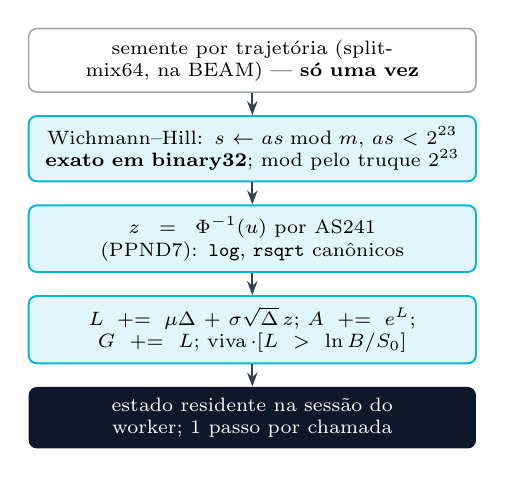
\begin{tikzpicture}[node distance=0.28cm]
  \node[box,text width=5.4cm] (s) {semente por trajetória (splitmix64, na BEAM) --- \textbf{só uma vez}};
  \node[acc,text width=5.4cm,below=of s] (w) {Wichmann--Hill: $s \leftarrow a s \bmod m$, $a s < 2^{23}$\\ \textbf{exato em binary32}; mod pelo truque $2^{23}$};
  \node[acc,text width=5.4cm,below=of w] (n) {$z = \Phi^{-1}(u)$ por AS241 (PPND7): \texttt{log}, \texttt{rsqrt} canônicos};
  \node[acc,text width=5.4cm,below=of n] (l) {$L \mathrel{+}= \mu\Delta + \sigma\sqrt{\Delta}\,z$;\ $A \mathrel{+}= e^{L}$;\ $G \mathrel{+}= L$;\ viva$\,\cdot$[$L>\ln B/S_0$]};
  \node[dark,text width=5.4cm,below=of l] (o) {estado residente na sessão do worker; 1 passo por chamada};
  \foreach \a/\b in {s/w,w/n,n/l,l/o} \draw[arr] (\a) -- (\b);
\end{tikzpicture}
\end{column}
\begin{column}{0.42\textwidth}
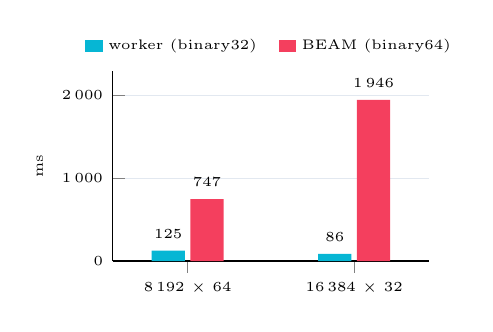
\begin{tikzpicture}
\begin{axis}[ybar, bar width=12pt, bar shift auto, width=5.6cm, height=4.0cm, ymin=0, ymax=2300,
  symbolic x coords={8\,192 $\times$ 64, 16\,384 $\times$ 32}, xtick=data, xticklabel style={font=\tiny}, enlarge x limits=0.45,
  yticklabel style={font=\tiny, /pgf/number format/1000 sep={\,}}, ylabel={ms}, ylabel style={font=\tiny},
  legend style={font=\tiny,at={(0.5,1.03)},anchor=south,draw=none,fill=none,legend columns=2,/tikz/every even column/.append style={column sep=6pt}},
  boxlegend,
  axis x line*=bottom, axis y line*=left, ymajorgrids, grid style={vmist},
  nodes near coords, nodes near coords style={font=\tiny, /pgf/number format/1000 sep={\,}, yshift=1pt}]
  \addplot[fill=vcyan,draw=none] coordinates {(8\,192 $\times$ 64,125) (16\,384 $\times$ 32,86)};
  \addplot[fill=vcoral,draw=none] coordinates {(8\,192 $\times$ 64,747) (16\,384 $\times$ 32,1946)};
  \legend{worker (binary32), BEAM (binary64)}
\end{axis}
\end{tikzpicture}\\[2pt]
{\tiny\renewcommand{\arraystretch}{1.1}
\begin{tabular}{@{}ll@{}}
oráculo (64 pistas) & \ok\ bits iguais\\
2 threads & \ok\ bits iguais\\
BSM em IC 99\% & \ok\ $z=1{,}17$\\
\textbf{controle}: sem Itô & \no\ $z=8{,}7$ --- pego\\
asiática c/ var. de controle & variância $\div$ 1\,300\\
\end{tabular}}
\end{column}
\end{columns}
\tese{Um número de risco que \hl{não muda com a máquina nem com as threads} --- e que diz isso na própria resposta.}
\end{frame}

\begin{frame}{Backtests: antecipação é propriedade de prefixo}
\begin{columns}[T]
\begin{column}{0.5\textwidth}
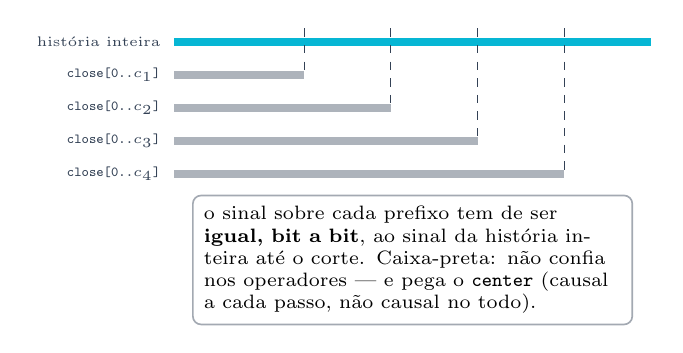
\begin{tikzpicture}[x=0.55cm,y=0.42cm]
  \foreach \c [count=\k] in {3,5,7,9} {
    \draw[vslate!40,line width=3pt] (0,-\k) -- (\c,-\k);
    \node[lbl,anchor=east] at (-0.1,-\k) {\texttt{close[0..}$c_{\k}$\texttt{]}};
  }
  \draw[vcyan,line width=3pt] (0,0) -- (11,0); \node[lbl,anchor=east] at (-0.1,0) {história inteira};
  \foreach \c [count=\k] in {3,5,7,9} \draw[dashed,vslate] (\c,0.4) -- (\c,-\k);
  \node[box,text width=5.3cm,align=left] at (5.5,-6.6) {o sinal sobre cada prefixo tem de ser \textbf{igual, bit a bit}, ao sinal da história inteira até o corte. Caixa-preta: não confia nos operadores --- e pega o \texttt{center} (causal a cada passo, não causal no todo).};
\end{tikzpicture}
\end{column}
\begin{column}{0.48\textwidth}
{\tiny\renewcommand{\arraystretch}{1.18}
\begin{tabular}{@{}p{2.25cm}cccc@{}}
\toprule
 & look-ahead & DSR & PBO & RC $p$\\
\midrule
ruído: melhor de 30 cruzamentos & \ok & \bad{0,10} & 0,24 & \bad{0,78}\\
plantado: AR(1), $\phi=0{,}15$ & \ok & \hl{1,00} & $<0{,}5$ & $<0{,}05$\\
\texttt{sign(lead(close)-close)} & \bad{dia 89} & --- & --- & ---\\
\texttt{sign(center(close))} & \bad{pego} & --- & --- & ---\\
\bottomrule
\end{tabular}}\\[6pt]
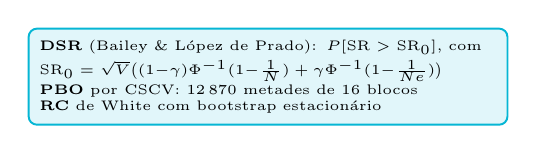
\begin{tikzpicture}
  \node[acc,text width=5.8cm,align=left,font=\tiny] {\textbf{DSR} (Bailey \& López de Prado): $P[\mathrm{SR} > \mathrm{SR}_0]$, com\\[1pt]$\mathrm{SR}_0 = \sqrt{V}\big((1{-}\gamma)\Phi^{-1}(1{-}\tfrac1N) + \gamma\Phi^{-1}(1{-}\tfrac{1}{Ne})\big)$\\
  \textbf{PBO} por CSCV: 12\,870 metades de 16 blocos\\ \textbf{RC} de White com bootstrap estacionário};
\end{tikzpicture}
\end{column}
\end{columns}
\tese{O Sharpe do trapaceiro é 20; o do ruído selecionado parece bom. \hl{Os portões dizem os dois}.}
\end{frame}

\begin{frame}{Arbitragem decidida pelo lema de Farkas}
\begin{columns}[T]
\begin{column}{0.5\textwidth}
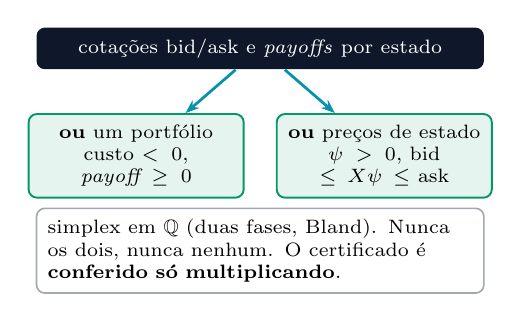
\begin{tikzpicture}
  \node[dark,text width=5.4cm] (q) {cotações bid/ask e \emph{payoffs} por estado};
  \node[goodb,text width=2.45cm,below left=0.55cm and -2.65cm of q] (a) {\textbf{ou} um portfólio\\ custo $<0$, \emph{payoff} $\ge 0$};
  \node[goodb,text width=2.45cm,below right=0.55cm and -2.65cm of q] (b) {\textbf{ou} preços de estado\\ $\psi > 0$, bid $\le X\psi \le$ ask};
  \draw[carr] (q) -- (a); \draw[carr] (q) -- (b);
  \node[box,text width=5.4cm,below=1.75cm of q,align=left] {simplex em $\mathbb{Q}$ (duas fases, Bland). Nunca os dois, nunca nenhum. O certificado é \textbf{conferido só multiplicando}.};
\end{tikzpicture}
\end{column}
\begin{column}{0.48\textwidth}
{\tiny\renewcommand{\arraystretch}{1.15}
\begin{tabular}{@{}p{2.3cm}p{3.4cm}@{}}
\toprule
cotações & veredito exato\\
\midrule
binomial coerente & $\psi = (1/2,\ 9/20)$\\
call a 14--14,5 & vender 1 título, comprar 1/90 da ação, vender 1/60 da call: \hl{recebe 1/15}, paga 0 nos dois estados\\
calls 90/100/110 & borboleta $\tfrac12 C_{90} - C_{100} + \tfrac12 C_{110}$: \hl{recebe 1/4}\\
câmbio USD/EUR/BRL & ciclo com produto $590000/584821 > 1$\\
\bottomrule
\end{tabular}}\\[6pt]
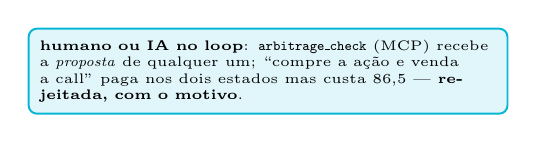
\begin{tikzpicture}
  \node[acc,text width=5.8cm,align=left,font=\tiny] {\textbf{humano ou IA no loop}: \texttt{arbitrage\_check} (MCP) recebe a \emph{proposta} de qualquer um; ``compre a ação e venda a call'' paga nos dois estados mas custa 86,5 --- \textbf{rejeitada, com o motivo}.};
\end{tikzpicture}
\end{column}
\end{columns}
\tese{Arbitragem não é estimada: é \hl{decidida}, e a decisão vem com o objeto que a prova.}
\end{frame}

\begin{frame}{O livro de ofertas como objeto verificável}
\centering
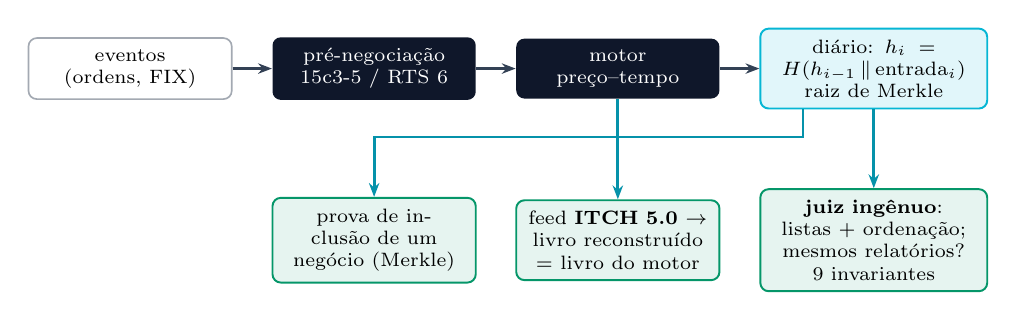
\begin{tikzpicture}[node distance=0.5cm]
  \node[box,text width=2.3cm] (e) {eventos\\ (ordens, FIX)};
  \node[dark,text width=2.3cm,right=of e] (g) {pré-negociação\\ 15c3-5 / RTS 6};
  \node[dark,text width=2.3cm,right=of g] (m) {motor\\ preço--tempo};
  \node[acc,text width=2.6cm,right=of m] (j) {diário: $h_i = H(h_{i-1}\,\Vert\,\text{entrada}_i)$\\ raiz de Merkle};
  \node[goodb,text width=2.6cm,below=1.0cm of j] (c) {\textbf{juiz ingênuo}: listas + ordenação; mesmos relatórios? 9 invariantes};
  \node[goodb,text width=2.3cm] (i) at (m |- c) {feed \textbf{ITCH 5.0} $\to$ livro reconstruído = livro do motor};
  \node[goodb,text width=2.3cm] (p) at (g |- c) {prova de inclusão de um negócio (Merkle)};
  \draw[arr] (e) -- (g); \draw[arr] (g) -- (m); \draw[arr] (m) -- (j); \draw[carr] (j) -- (c); \draw[carr] (m) -- (i);
  \draw[carr] (j.south) ++(-0.9,0) coordinate (js) -- ++(0,-0.35) -| (p.north);
\end{tikzpicture}\\[6pt]
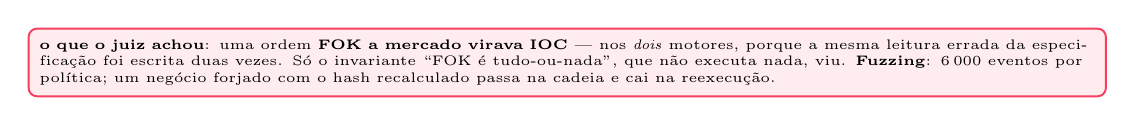
\begin{tikzpicture}
  \node[badb,text width=13.4cm,align=left,font=\tiny] {\textbf{o que o juiz achou}: uma ordem \textbf{FOK a mercado virava IOC} --- nos \emph{dois} motores, porque a mesma leitura errada da especificação foi escrita duas vezes. Só o invariante ``FOK é tudo-ou-nada'', que não executa nada, viu. \textbf{Fuzzing}: 6\,000 eventos por política; um negócio forjado com o hash recalculado passa na cadeia e cai na reexecução.};
\end{tikzpicture}
\tese{Dois motores não bastam: \hl{os invariantes são o terceiro juiz}. E o backtest roda o código da bolsa, não um modelo dela.}
\end{frame}

\begin{frame}{Microestrutura: cada modelo com a sua medida}
\begin{columns}[T]
\begin{column}{0.33\textwidth}
\textbf{\small Hawkes}\\[2pt]
{\tiny plantado $(\mu,\alpha,\beta) = (1;\,0{,}6;\,1{,}5)$\\ ajustado $(1{,}08;\,0{,}61;\,1{,}69)$\\ ramificação 0,36 (0,40)\\[3pt]
\begin{tabular}{@{}lc@{}}
\toprule
teste de reescala & KS $p$\\ \midrule
Hawkes & \hl{0,73}\\ Poisson (controle) & \bad{$1{,}7\cdot10^{-20}$}\\ \bottomrule
\end{tabular}}
\end{column}
\begin{column}{0.33\textwidth}
\textbf{\small Avellaneda--Stoikov}\\[2pt]
{\tiny $\gamma=0{,}1$, 1\,000 trajetórias, §4 do artigo\\[3pt]
\begin{tabular}{@{}lcc@{}}
\toprule
 & daqui & artigo\\ \midrule
$\sigma$(P\&L) estoque & 6,44 & 5,89\\
$\sigma$(P\&L) simétrica & 13,57 & 13,43\\
$\sigma(q)$ estoque & 2,97 & 2,80\\
$\sigma(q)$ simétrica & 8,37 & 8,66\\ \bottomrule
\end{tabular}}
\end{column}
\begin{column}{0.32\textwidth}
\textbf{\small Almgren--Chriss}\\[2pt]
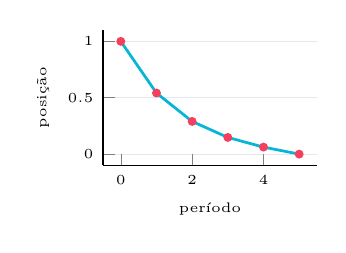
\begin{tikzpicture}
\begin{axis}[width=4.3cm,height=3.3cm,xlabel={período},ylabel={posição},xlabel style={font=\tiny},ylabel style={font=\tiny},ticklabel style={font=\tiny},axis x line*=bottom,axis y line*=left,ymajorgrids,grid style={vmist}]
  \addplot[vcyan,line width=1pt] coordinates {(0,1) (1,0.54196) (2,0.28985) (3,0.14790) (4,0.06214) (5,0)};
  \addplot[only marks,mark=*,mark size=1.4pt,vcoral] coordinates {(0,1) (1,0.54196) (2,0.28985) (3,0.14790) (4,0.06214) (5,0)};
\end{axis}
\end{tikzpicture}
\\[-1pt]{\tiny fechada (linha) = numérica (pontos): $10^{-16}$}
\end{column}
\end{columns}
\tese{Um modelo de microestrutura sem o seu teste é uma história; \hl{com o teste e o controle, é uma medida}.}
\end{frame}

\begin{frame}{Pendências fechadas e o que fica aberto}
\begin{columns}[T]
\begin{column}{0.5\textwidth}
{\tiny\renewcommand{\arraystretch}{1.2}
\begin{tabular}{@{}p{2.2cm}p{3.9cm}@{}}
\toprule
\textbf{pendência} & \textbf{fechada como}\\ \midrule
LP com Farkas & simplex em $\mathbb{Q}$: dual, Farkas, raio; = HiGHS a $10^{-9}$\\
arquivos assinados & Ed25519 sobre o manifesto; a mentira coerente recusada\\
°C / °F & leituras afins; 98,6 °F = 37 °C; compostas recusadas\\
transistores & MOSFET nível 1 e Ebers--Moll \hl{= ngspice na 6ª casa}\\
\bottomrule
\end{tabular}}
\end{column}
\begin{column}{0.48\textwidth}
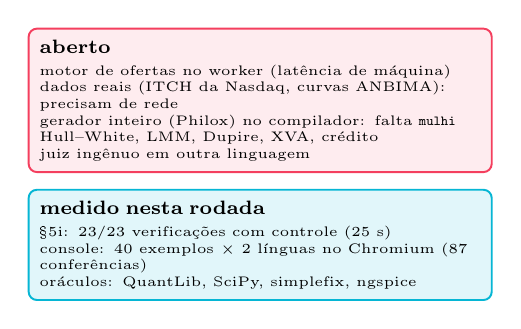
\begin{tikzpicture}
  \node[badb,text width=5.6cm,align=left,font=\tiny] (a) {\textbf{\scriptsize aberto}\\[2pt]
    motor de ofertas no worker (latência de máquina)\\
    dados reais (ITCH da Nasdaq, curvas ANBIMA): precisam de rede\\
    gerador inteiro (Philox) no compilador: falta \texttt{mulhi}\\
    Hull--White, LMM, Dupire, XVA, crédito\\
    juiz ingênuo em outra linguagem};
  \node[acc,text width=5.6cm,align=left,font=\tiny,below=0.2cm of a] {\textbf{\scriptsize medido nesta rodada}\\[2pt]
    §5i: 23/23 verificações com controle (25 s)\\
    console: 40 exemplos $\times$ 2 línguas no Chromium (87 conferências)\\
    oráculos: QuantLib, SciPy, simplefix, ngspice};
\end{tikzpicture}
\end{column}
\end{columns}
\tese{As pendências fechadas são as que o domínio novo \hl{tornou necessárias}: o simplex decide a arbitragem; a assinatura faz de uma sessão um registro.}
\end{frame}

\begin{frame}{0.14: de vitrine a ferramenta}
\centering
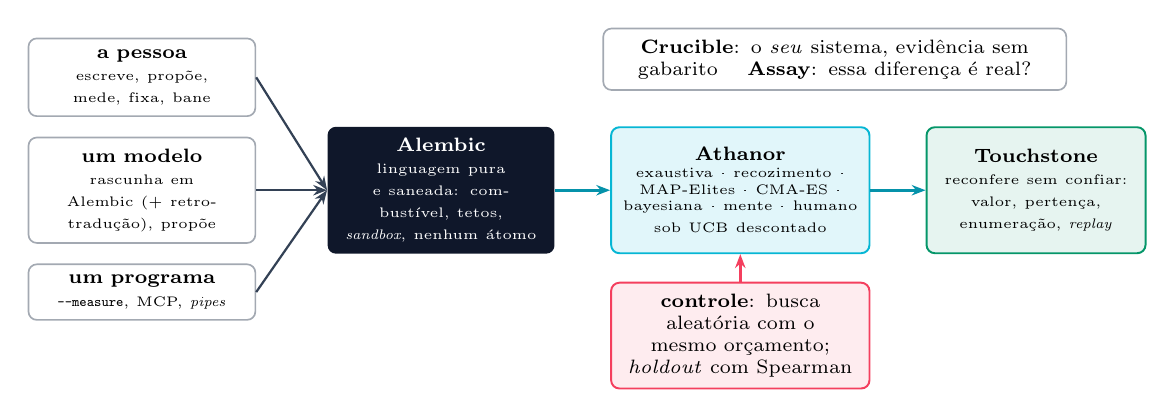
\begin{tikzpicture}[node distance=0.35cm and 0.5cm]
  \node[box,text width=2.6cm] (p) {\textbf{a pessoa}\\{\tiny escreve, propõe, mede, fixa, bane}};
  \node[box,text width=2.6cm,below=0.25cm of p] (m) {\textbf{um modelo}\\{\tiny rascunha em Alembic (+ retrotradução), propõe}};
  \node[box,text width=2.6cm,below=0.25cm of m] (x) {\textbf{um programa}\\{\tiny \texttt{--measure}, MCP, \emph{pipes}}};
  \node[dark,text width=2.6cm,right=0.9cm of m,minimum height=1.6cm] (a) {\textbf{Alembic}\\{\tiny linguagem pura e saneada: combustível, tetos, \emph{sandbox}, nenhum átomo}};
  \node[acc,text width=3.0cm,right=0.7cm of a,minimum height=1.6cm] (f) {\textbf{Athanor}\\{\tiny exaustiva · recozimento · MAP-Elites · CMA-ES · bayesiana · mente · humano\\ sob UCB descontado}};
  \node[goodb,text width=2.5cm,right=0.7cm of f,minimum height=1.6cm] (t) {\textbf{Touchstone}\\{\tiny reconfere sem confiar: valor, pertença, enumeração, \emph{replay}}};
  \node[badb,text width=3.0cm,below=0.35cm of f] (c) {\textbf{controle}: busca aleatória com o mesmo orçamento; \emph{holdout} com Spearman};
  \foreach \n in {p,m,x} \draw[arr] (\n.east) -- (a.west);
  \draw[carr] (a) -- (f); \draw[carr] (f) -- (t); \draw[rarr] (c) -- (f);
  \node[box,text width=5.6cm,above=0.45cm of f,xshift=1.2cm] (cr) {\textbf{Crucible}: o \emph{seu} sistema, evidência sem gabarito \quad \textbf{Assay}: essa diferença é real?};
\end{tikzpicture}\\[4pt]
{\scriptsize os buscadores famosos são casos de \emph{proponha $\to$ avalie $\to$ certifique}: o produto é o caso geral, e os casos viram \textbf{exemplos} (Golomb, Ramsey, redes de ordenação, portfólios, hiperparâmetros, regras de \emph{trading}, fórmulas)}
\tese{Ninguém escolhe de uma lista: \hl{escreve o problema}. O modelo propõe; \hl{quem decide é o verificador} --- o mesmo para a pessoa, o modelo e o acaso.}
\end{frame}

\begin{frame}{Athanor: a fornalha contra o acaso}
\begin{columns}[T]
\begin{column}{0.56\textwidth}
{\tiny\renewcommand{\arraystretch}{1.25}
\begin{tabular}{@{}p{2.4cm}p{1.75cm}p{2.15cm}@{}}
\toprule
\textbf{problema} & \textbf{fornalha} & \textbf{controle}\\ \midrule
Golomb, 7 marcas & \hl{25 (ótimo)} & aleatório: \bad{0} acertos em 3\,923\\
max-cut, $2^{10}$ cortes & 13, \hl{exaurido} & força bruta independente: 13; forjado 14: \bad{recusado}\\
$R(3,3)=6$ & \hl{provado} em 32\,768 grafos & $K_5$: o pentágono refuta\\
Euler (somas de potências) & contraexemplo em 40 & ---\\
médias móveis, \emph{holdout} & AR(1) $\varphi=0{,}5$: $\rho=$ \hl{0,73} & passeio aleatório: $\rho=$ \bad{$-0{,}33$}\\
\emph{replay} & mesma semente, mesma raiz & semente 2: outra raiz\\
\bottomrule
\end{tabular}}
\end{column}
\begin{column}{0.42\textwidth}
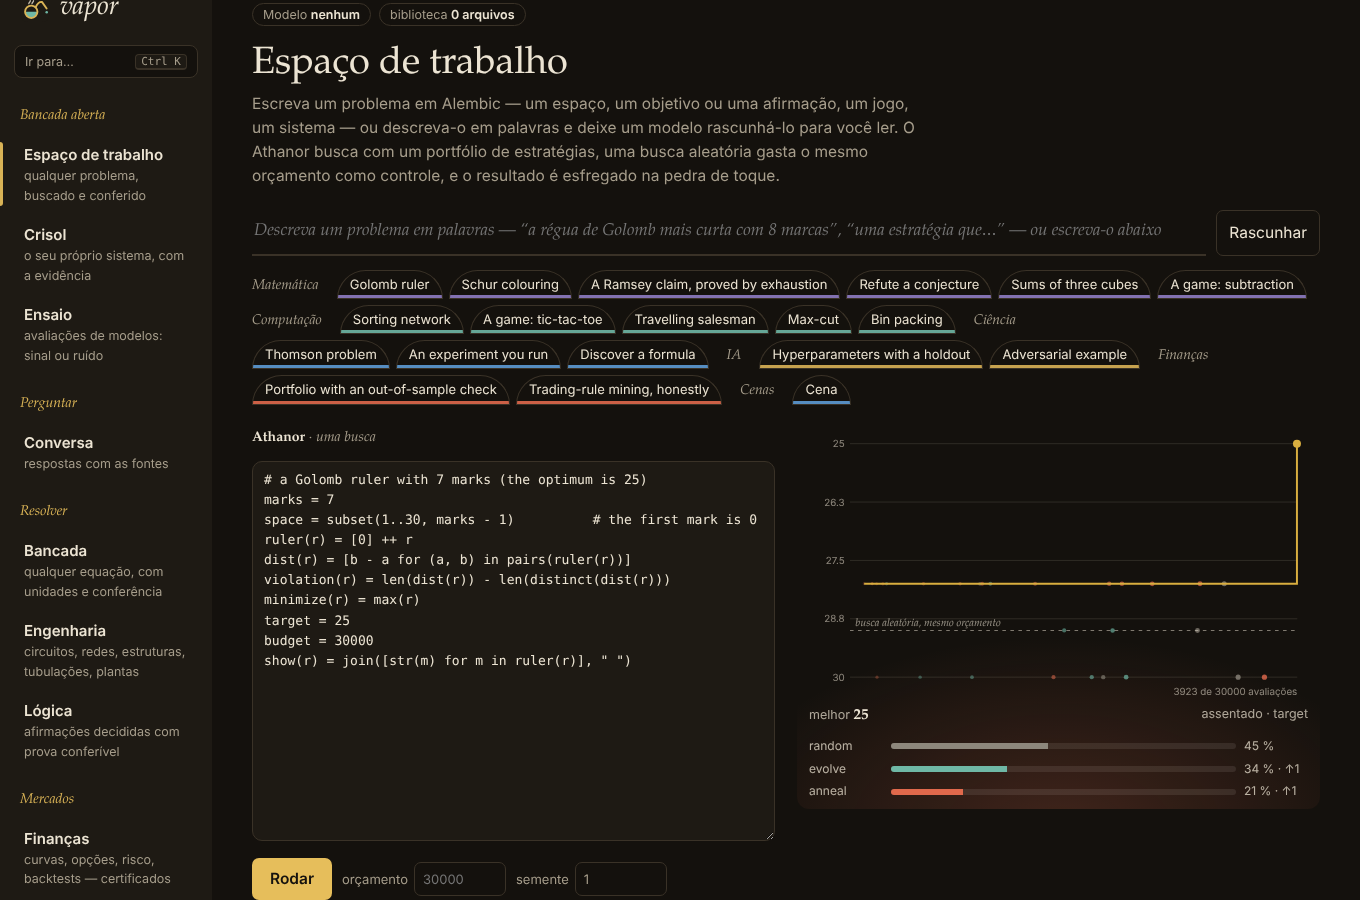
\includegraphics[width=\linewidth]{../docs/img/bancada-athanor-escuro.png}\\[-2pt]
{\tiny a fornalha ao vivo: faíscas por avaliação, a linha do melhor, a tracejada do controle, a partilha do portfólio}
\end{column}
\end{columns}
\tese{``Provado'' quer dizer \hl{enumeração completa de um espaço finito}, com o tamanho no certificado; o resto é evidência, e o \emph{holdout} diz quando é viés de seleção.}
\end{frame}

\begin{frame}{Crucible e Assay: evidência sem gabarito; sinal ou ruído}
\begin{columns}[T]
\begin{column}{0.5\textwidth}
\textbf{\small Crucible} {\tiny (o sistema é da pessoa)}\\[3pt]
{\tiny\renewcommand{\arraystretch}{1.2}
\begin{tabular}{@{}p{2.3cm}p{1.45cm}p{1.6cm}@{}}
\toprule
& valor & controle\\ \midrule
6 hamiltonianos cúbicos aleatórios & H \hl{6/6} provado sobre $\mathbb{Q}$ & dissipativos: \hl{0} leis\\
oscilador quântico & $|E-(n+\frac12)|$ $3\cdot10^{-6}$, ordem 1,99 & caixa pequena: evidência \bad{falha}\\
Kepler, 250 órbitas & Yoshida: $\le 1{,}4\cdot10^{-3}$ & RK4: \bad{0,062}\\
H$_2$ RHF/STO-3G & \hl{$-1{,}1167$} & esticado: acima de 2 H (falha do RHF, exibida)\\
regressão simbólica & $R^2=1{,}0$ & alvo embaralhado: $-0{,}32$\\
\bottomrule
\end{tabular}}
\end{column}
\begin{column}{0.48\textwidth}
\textbf{\small Assay} {\tiny (pesquisa em IA)}\\[3pt]
{\tiny\renewcommand{\arraystretch}{1.2}
\begin{tabular}{@{}p{1.9cm}p{1.55cm}p{1.65cm}@{}}
\toprule
& valor & controle\\ \midrule
comparação pareada & erro tipo I \hl{0,00} em 60 nulos & efeito plantado: $p=2{,}5\cdot10^{-4}$\\
calibração & calibrado: $p=0{,}45$ & confiante: $p=$ \bad{0,002}; Platt 0,23$\to$0,08\\
Krippendorff & \hl{0,743} (publicado) & ao acaso: 0,007\\
lei de escala & $\alpha\in[0{,}334;\,0{,}351]$, erro 0,3\,\% & perdas embaralhadas: \bad{33\,\%}\\
\bottomrule
\end{tabular}}\\[4pt]
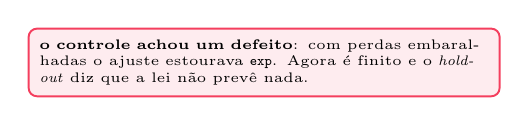
\begin{tikzpicture}\node[badb,text width=5.7cm,align=left,font=\tiny] {\textbf{o controle achou um defeito}: com perdas embaralhadas o ajuste estourava \texttt{exp}. Agora é finito e o \emph{holdout} diz que a lei não prevê nada.};\end{tikzpicture}
\end{column}
\end{columns}
\tese{A pergunta mais comum da pesquisa em IA não é ``como treinar'': é \hl{``essa diferença é real?''}.}
\end{frame}

\begin{frame}[fragile]{Tudo pelo terminal, pela mesma porta}
\begin{columns}[T]
\begin{column}{0.56\textwidth}
{\tiny
\begin{verbatim}
$ vapor athanor run euler.alb > c.json   # sai 1: refutada
$ vapor verify euler.alb c.json --replay # sai 0: conferido
$ echo "régua de Golomb com 8 marcas" \
    | vapor mind formalize - > g.alb     # + retrotradução
$ vapor athanor run hp.alb --measure ./treina.sh
$ vapor crucible laws sir.txt | jq '.laws[].law'
$ vapor assay compare evals.csv && echo real
$ vapor scene edit s.json "add glow sol { x: 0.7 }"
\end{verbatim}}
{\tiny JSON em \emph{pipes}; saídas 0 positivo · 1 negativo · 2 uso · 3 entrada · 4 falha}
\end{column}
\begin{column}{0.42\textwidth}
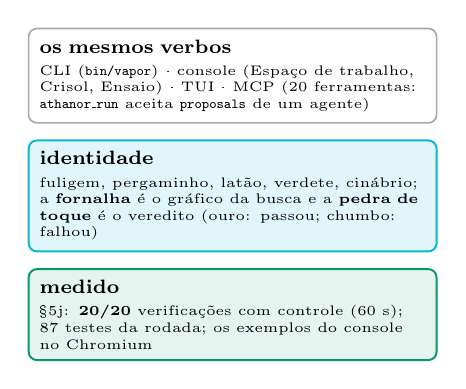
\begin{tikzpicture}
  \node[box,text width=4.9cm,align=left,font=\tiny] (a) {\textbf{\scriptsize os mesmos verbos}\\[2pt]
    CLI (\texttt{bin/vapor}) · console (Espaço de trabalho, Crisol, Ensaio) · TUI · MCP (20 ferramentas: \texttt{athanor\_run} aceita \texttt{proposals} de um agente)};
  \node[acc,text width=4.9cm,align=left,font=\tiny,below=0.2cm of a] (b) {\textbf{\scriptsize identidade}\\[2pt]
    fuligem, pergaminho, latão, verdete, cinábrio; a \textbf{fornalha} é o gráfico da busca e a \textbf{pedra de toque} é o veredito (ouro: passou; chumbo: falhou)};
  \node[goodb,text width=4.9cm,align=left,font=\tiny,below=0.2cm of b] {\textbf{\scriptsize medido}\\[2pt]
    §5j: \textbf{20/20} verificações com controle (60 s); 87 testes da rodada; os exemplos do console no Chromium};
\end{tikzpicture}
\end{column}
\end{columns}
\tese{Nenhuma capacidade existe só na interface gráfica: \hl{o console é um cliente do terminal}, não o contrário.}
\end{frame}

\begin{frame}{0.15: o Opus --- decidir, não exibir}
{\tiny\renewcommand{\arraystretch}{1.3}
\begin{tabular}{@{}p{1.6cm}p{4.4cm}p{3.1cm}p{3.6cm}@{}}
\toprule
\textbf{peça} & \textbf{primeiro princípio} & \textbf{valor} & \textbf{controle}\\ \midrule
Amálgama & todo binário é inteiro $\times\,2^{q_{\min}}$: soma de inteiros é associativa (Kulisch na BEAM) & \hl{1} resultado em 30 ordens, = soma exata arredondada uma vez & esquerda $\to$ direita: \bad{30} resultados\\
Copela & $y\cdot r = x\cdot(W^{\top} r)$ em aritmética exata; tolerância de Higham \emph{provada} & bits 19--31: \hl{100\,\%}; 0 acusações em 24 ordens conformes & bit 0: 0\,\% (abaixo do envelope, \emph{dito})\\
Rebis & a ANF \emph{é} a forma normal (Möbius); Gröbner sobre $\mathbb{Z}$ para palavras & cavalo de Troia de 32 bits: \hl{0xDEADBEEF}; multiplicador 32 bits em 1,4\,s & 4\,096 padrões aleatórios: \bad{não viram}\\
Aludel & Bernstein + de Casteljau em inteiros; três vereditos (do PALADIN) & Motzkin $+\frac{1}{1000}>0$: \hl{certificado}, testemunha reproduzida & Motzkin $\ge 0$: \bad{esgotado}, não fingido\\
Tábua & antinomia = cenário satisfazível; consistência = prova DRUP & C1 $\times$ C6 com o cenário; C1 $\times$ C3 \hl{provado} & com as precedências: 0 antinomias\\
\bottomrule
\end{tabular}}\\[4pt]
{\scriptsize e dois caminhos antes recusados, fechados: \textbf{JBIG2 Huffman e meio-tom} (64 fixtures, um defeito do jbig2dec registrado) e o \textbf{alinhamento antes da fusão} (Git Re-Basin, húngaro exato: a cópia embaralhada volta a ser a rede)}
\tese{Cada peça devolve um \hl{veredito que se confere sem confiar nela} --- e diz o que não vê.}
\end{frame}

\begin{frame}{0.15: o pedido escrutinado}
\begin{columns}[T]
\begin{column}{0.5\textwidth}
{\tiny
\textbf{\scriptsize os anexos, fagocitados como ideias}\\[3pt]
\begin{tabular}{@{}p{1.3cm}p{3.9cm}@{}}
\toprule
PALADIN & $\to$ \hl{Aludel}, quase inteiro\\
WIZARD & ordem declarada $\to$ \hl{Amálgama}: a ordem deixa de importar\\
GHOST & quórum $3f{+}1$ $\to$ \hl{Copela}: conferir em vez de votar\\
JESTER & raiz de época = o diário Merkle que já existia\\
HYDRA-Z & NCD não é métrica com compressores reais; LSH já evita os $O(N^2)$ pares\\
\bottomrule
\end{tabular}}
\end{column}
\begin{column}{0.48\textwidth}
{\tiny
\textbf{\scriptsize achado no caminho}\\[2pt]
\texttt{dot16} truncava a cauda em silêncio; o teste de auditoria e um de figuras já falhavam na 0.14 (\texttt{System.cmd}; corrida em \texttt{/dev/shm}); 15 funções sem chamador.\\[5pt]
\textbf{\scriptsize recusado, com o motivo}\\[2pt]
\bad{``permutação isomórfica''} para ficar abaixo dos limiares de plágio (evasão de detecção); ``certificado de não-infringência em Lean''; Merkle provando \emph{ausência} de dados; ``resolver'' a paisagem das cordas.}
\end{column}
\end{columns}
\tese{Reescrever 88 mil linhas destruiria a continuidade da evidência: \hl{reengenharia onde o primeiro princípio muda a resposta}, e só ali.}
\end{frame}

\begin{frame}{0.16: purificar --- conversar, um terminal, uma balança}
{\tiny\renewcommand{\arraystretch}{1.3}
\begin{tabular}{@{}p{1.6cm}p{4.4cm}p{3.1cm}p{3.6cm}@{}}
\toprule
\textbf{peça} & \textbf{primeiro princípio} & \textbf{valor} & \textbf{controle}\\ \midrule
Khazāna & conteúdo imutável + raiz em dois slots com sequência e etiqueta (ASAS §8.4) & queda em \hl{cada byte} de um \emph{commit}: raiz velha ou nova & arquivo único sobrescrito: \bad{lê v2 rasgado}\\
Majlis & a conversa é uma árvore; o hash da mensagem cobre o pai & bifurcar: \hl{0} mensagens copiadas; um caractere trocado: recusado & cópia profunda: 120; Markdown: \bad{não vê}\\
Contexto & calculado e mostrado: fixadas + último turno + as mais novas que cabem & instrução fixada e pergunta: \hl{enviadas} & truncar pela cauda: \bad{perde a instrução}\\
Dīwān & um interpretador para CLI, TUI, console e API; jaula no console & ler arquivo do servidor: \hl{recusado} & sessão local: lê\\
Mīzān & árvore neutra, duas escritas bijetivas; obrigações por decisores & conservação \hl{provada} sobre $\mathbb{Q}$; amortecida $10^{-9}$ refutada & amostrar $\dot H$: \bad{aceita a amortecida}\\
Geometria & Fisher--Rao é métrica; gradiente natural é invariante & 0 violações; $7\cdot10^{-12}$ & KL: \bad{217}; gradiente simples: \bad{0,54}\\
\bottomrule
\end{tabular}}\\[4pt]
{\scriptsize saíram: redes complexas, descoberta de algoritmos, jogo da velha, dez painéis de demonstração --- \textbf{2\,949 linhas}; ficou o que responde a uma pergunta com os dados de quem pergunta}
\tese{Superar um produto de conversa não é prometer um modelo melhor: é tratar a conversa como \hl{objeto verificável}.}
\end{frame}

\begin{frame}{0.16: o manifesto Al-Mīzān e as três críticas}
\begin{columns}[T]
\begin{column}{0.5\textwidth}
{\tiny
\textbf{\scriptsize pesado item a item}\\[3pt]
\begin{tabular}{@{}p{1.6cm}p{3.6cm}@{}}
\toprule
raízes, \emph{awzān} & \hl{mantidos}: domínio e regime como tipo morfológico\\
árabe RTL & \hl{projeção} bijetiva, não a linguagem; o mesmo hash\\
\emph{abjad} & \bad{refutado}: 99,99\,\% das raízes colidem\\
Lean & \hl{decisores} primeiro ($\mathbb{Q}$, Bernstein, SAT+DRUP); Lean como 2ª opinião\\
\texttt{.mzn} & a raiz é \emph{w-z-n} (pesar); \texttt{.mzn} é do MiniZinc $\to$ \hl{\texttt{.wzn}}\\
\bottomrule
\end{tabular}}
\end{column}
\begin{column}{0.48\textwidth}
{\tiny
\textbf{\scriptsize as críticas}\\[2pt]
\textbf{Riemann × hardware discreto}: roda-se a fórmula fechada (uma soma e um arco-cosseno), não a variedade; e só onde há distribuição.\\[3pt]
\textbf{dependência de ITP}: cada obrigação enunciável tem um decisor; \emph{desconhecido} não compila.\\[3pt]
\textbf{sintaxe × semântica}: a semântica mora na árvore; raiz e \emph{wazn} sobrevivem a qualquer escrita.\\[5pt]
\textbf{\scriptsize Alembic e vapor}: ASCII --- leitores do mundo todo, em diffs e terminais. \textbf{\scriptsize Mīzān}: dialeto \emph{declarado}, não secreto.}
\end{column}
\end{columns}
\tese{A balança pesa o que os seus decisores decidem --- e \hl{recusa o resto}.}
\end{frame}

% =========================================================================
\section{8 · Contribuição}
% =========================================================================
\begin{frame}{Legado: o que fica, com a evidência de cada item}
\begin{columns}[T]
\begin{column}{0.64\textwidth}
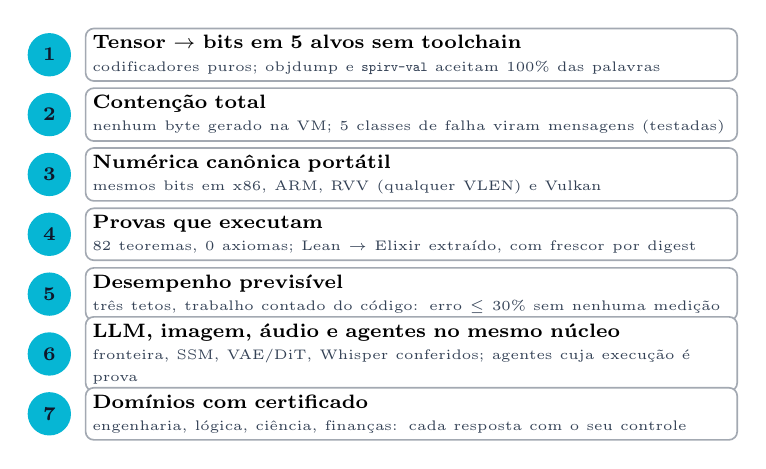
\begin{tikzpicture}[num/.style={circle,fill=vcyan,text=vnavy,font=\scriptsize\bfseries,minimum size=0.55cm,inner sep=0},
                    it/.style={box,text width=8.1cm,align=left,anchor=west,minimum height=0.66cm,inner sep=2.5pt}]
  \foreach \t/\e [count=\ix] in {
    {Tensor $\to$ bits em 5 alvos sem toolchain}/{codificadores puros; objdump e \texttt{spirv-val} aceitam 100\% das palavras},
    {Contenção total}/{nenhum byte gerado na VM; 5 classes de falha viram mensagens (testadas)},
    {Numérica canônica portátil}/{mesmos bits em x86, ARM, RVV (qualquer VLEN) e Vulkan},
    {Provas que executam}/{82 teoremas, 0 axiomas; Lean $\to$ Elixir extraído, com frescor por digest},
    {Desempenho previsível}/{três tetos, trabalho contado do código: erro $\le$ 30\% sem nenhuma medição},
    {LLM, imagem, áudio e agentes no mesmo núcleo}/{fronteira, SSM, VAE/DiT, Whisper conferidos; agentes cuja execução é prova},
    {Domínios com certificado}/{engenharia, lógica, ciência, finanças: cada resposta com o seu controle}} {
    \pgfmathsetmacro{\y}{-0.76*\ix}
    \node[num] at (0,\y) {\ix};
    \node[it] at (0.45,\y) {\textbf{\t}\\{\tiny\color{vslate}\e}};
  }
\end{tikzpicture}
\end{column}
\begin{column}{0.34\textwidth}
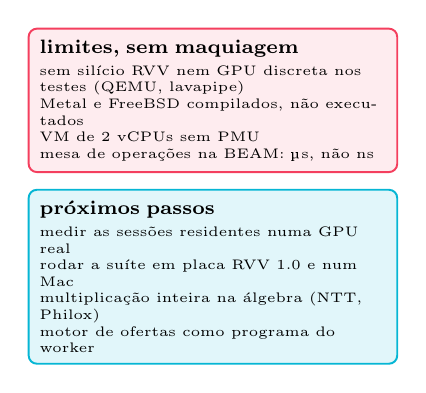
\begin{tikzpicture}
  \node[badb,text width=4.4cm,align=left,font=\tiny] (l) {\textbf{\scriptsize limites, sem maquiagem}\\[2pt]
    sem silício RVV nem GPU discreta nos testes (QEMU, lavapipe)\\
    Metal e FreeBSD compilados, não executados\\
    VM de 2 vCPUs sem PMU\\
    mesa de operações na BEAM: µs, não ns};
  \node[acc,text width=4.4cm,align=left,font=\tiny,below=0.2cm of l] {\textbf{\scriptsize próximos passos}\\[2pt]
    medir as sessões residentes numa GPU real\\
    rodar a suíte em placa RVV 1.0 e num Mac\\
    multiplicação inteira na álgebra (NTT, Philox)\\
    motor de ofertas como programa do worker};
\end{tikzpicture}
\end{column}
\end{columns}
\tese{A contribuição permanente não é velocidade: é mostrar que um compilador de tensores pode ser \hl{pequeno, isolado, portátil bit a bit --- e carregar a própria prova}.}
\end{frame}

\end{document}
